\RequirePackage{plautopatch}
\documentclass[dvipdfmx,uplatex,report]{jsbook} % \documentclass[a4paper]{jsreport}
\RequirePackage[l2tabu, orthodox]{nag} % 古いコマンド, パッケージに対する警告
\usepackage{amsmath, amssymb, amsfonts, amsthm}
\usepackage{ascmac}
\usepackage{bbm}
\usepackage{bigdelim}
\usepackage{cases}
\usepackage{chngcntr}
\usepackage[usenames]{color}
\usepackage{comment}
\usepackage{currfile}
\usepackage{empheq}
\usepackage{fancybox}
\usepackage{graphicx}
\usepackage{here}
\usepackage[dvipdfmx,colorlinks,linkcolor=Blue,urlcolor=blue,bookmarksopenlevel=4]{hyperref}
\usepackage{ifthen}
\usepackage{mathtools}
\usepackage{multirow}
\usepackage{nameref}
\usepackage{pxjahyper}
\usepackage{siunitx}
\usepackage{tabularx, arydshln}
\usepackage{udline}
\usepackage{url}
\usepackage{zref-xr}

% cross reference
\zxrsetup{toltxlabel} % use normal LaTeX style \ref
\zexternaldocument*[1:]{reference/Mathematics_Memorandum_v0.12.0} % usage: \zexternaldocument*[prefix]{path/to/aux/file/without/extension}[path/to/pdf/file] Only ascii name is allowed.

\theoremstyle{definition} % 定理環境:斜体なし
\newtheorem*{commentary}{解説}
\newtheorem*{attention}{注意}
\newtheorem*{solution}{解法}
\newtheorem*{definition}{定義}
\makeatletter
\newcounter{subsubsubsection}
\setcounter{subsubsubsection}{0}
\newcommand{\subsubsubsection}{
	\refstepcounter{subsubsubsection}
	\@startsection{paragraph}{4}{\z@}%
	{1.0\Cvs \@plus.5\Cdp \@minus.2\Cdp}%
	{.1\Cvs \@plus.3\Cdp}%
	{\reset@font\sffamily\normalsize}
}
\makeatother
\setcounter{secnumdepth}{4}

% section, subsection, subsubsection の先頭に部番号が付くようにする
\makeatletter
\@addtoreset{chapter}{part}\renewcommand{\thechapter}{\thepart.\arabic{chapter}}
\@addtoreset{section}{chapter}\renewcommand{\thesection}{\thechapter.\arabic{section}}
\@addtoreset{subsection}{section}\renewcommand{\thesubsection}{\thesection.\arabic{subsection}}
\@addtoreset{subsubsection}{subsection}\renewcommand{\thesubsubsection}{\thesubsection.\arabic{subsubsection}}
\@addtoreset{subsubsubsection}{subsubsection}\renewcommand{\thesubsubsubsection}{\thesubsubsection.\arabic{subsubsubsection}}

\renewcommand{\theequation}{\arabic{equation}} % jsbook によって書き換えられた \theequation を元に戻す

% section 毎に数式, 図番号をリセットする。番号表示は「part.chapter.section.section内での通し番号」となる。
\counterwithin{equation}{section}
\counterwithin{figure}{section}

% 目次の番号とタイトルが重ならないようにする
% dottedtocline{A}{B}{C}のパラメータABC
%   A:目次を生成するレベル(\chapterはレベル0、\sectionはレベル1...)
%   B:一番外側からの左マージン
%   C:見出し番号が入るボックスの幅
\renewcommand{\l@chapter}{\@dottedtocline{0}{0em}{7em}}
\renewcommand{\l@section}{\@dottedtocline{1}{1em}{7em}}
\renewcommand{\l@subsection}{\@dottedtocline{2}{2em}{6em}}
\renewcommand{\l@subsubsection}{\@dottedtocline{3}{3em}{5em}}
\makeatother

\setcounter{tocdepth}{4} % subsubsubsection まで目次に表示する

% document version number
\def\docVerMajor{0}
\def\docVerMinor{7}
\def\docVerPatch{0}
\def\docVerWip{} % \def\docVerWip{-wip}
\def\docVer{\docVerMajor.\docVerMinor.\docVerPatch\docVerWip}

\input{macros/LaTeX-motchyMacros/motchyMacros}

\begin{document}
	\title{信号処理備忘録}
	\author{motchy}
	\date{\西暦 2019年11月16日 $\sim$ \today \\ver \docVer}
	\maketitle
	{\scriptsize \tableofcontents}

	 \part{表記法}
		\chapter{数学記号}
			\begin{itemize}
				\item $\field$: 体
				\item $\integers$: 整数全体の集合
				\item $\realSpace$: 実数全体の集合
				\item $\complexSpace$: 複素数全体の集合
				\item $\bm{a}/\bm{b}\;(d \in \naturalNumbers,\;\bm{a},\bm{b} \in \field^d,\;b_i\neq 0 \text{ for all }i)$: $[a_1/b_1,\cdots,a_d/b_d]^\top$
				\item $a\%b\;(a,b\in\integers,\;b\neq 0)$: $a$を$b$で割った余り。符号に2通り考えられるが、本書では結果を0以上$|a|$未満とする定義を採用する。
				\item $\bm{a}\%\bm{b}\;(d\in\naturalNumbers,\;\bm{a},\bm{b} \in \integers^d,\; b_i\neq 0 \text{ for all }i)$: $[a_1\%b_1,\cdots,a_d\%b_d]^\top$
			\end{itemize}
		
		\chapter{連続座標信号の表現}
			連続的な座標値$\bm{x}\in\realSpace^{d_1}\;(d_1\in\naturalNumbers)$から$\realSpace^{d_2}\;(d_2\in\naturalNumbers)$への写像を$d_1$次元連続座標信号という。
			信号値は全ての座標に対して定義される必要はない。
			\par
			例えばカセットテープレコーダーに記録された音声信号は$d_1=d_2=1$のものである。
			\par
			信号$f$の位置$\bm{x} = [x_1,x_2,\cdots,x_{d_1}]^\top$での値を$f(\bm{x})$や$f(x_1,\cdots,x_{d_1})$で表す。

		\chapter{離散座標信号の表現}
			離散的な座標値$\bm{x}\in\integers^{d_1}\;(d_1\in\naturalNumbers)$から$\realSpace^{d_2}\;(d_2\in\naturalNumbers)$への写像を$d_1$次元離散座標信号という。
			信号値は全ての座標に対して定義される必要はない。
			\par
			例えば離散的な時刻での電圧のサンプリングデータは$d_1=d_2=1$のものである(この場合の「座標」は時間軸上での座標という意味になる)。
			また、コンピュータのディスプレイに映る2次元カラー画像は$d_1=2,d_2=3$のものである。
			\par
			信号$f$の位置$\bm{x} = [x_1,x_2,\cdots,x_{d_1}]^\top$での値を$f(\bm{x})$や$f(x_1,\cdots,x_{d_1})$で表す。

	\part{畳み込み}
	\chapter{畳み込みの微分}
		\section{関係式}
			\begin{shadebox}
				微分可能な複素数値信号 $x_1, x_2:\realNumbers\to\complexNumbers$ に畳み込みが存在するとき、次が成り立つ。
				\[ \derivLong{(x_1*x_2)(t)}{t}{} = {x_1}'*x_2 = x_1*{x_2}' \]
			\end{shadebox}
			\begin{proof}
				\quad\par
				まず次式が成り立つ。
				\begin{align*}
					\derivLong{(x_1*x_2)(t)}{t}{} &= \derivLong{\integrate{-\infty}{\infty}{x_1(\tau)x_2(t-\tau)}{}{\tau}}{t}{} = \integrate{-\infty}{\infty}{x_1(\tau)\derivLong{x_2(t-\tau)}{t}{}}{}{\tau} \\
					&= \integrate{-\infty}{\infty}{x_1(\tau){x_2}'(t-\tau)}{}{\tau} = (x_1*{x_2}')(t)
				\end{align*}
				$x_1*x_2 = x_2*x_1$ を用いて上記と同様の計算を行うと次式が成り立つ。
				\[ \derivLong{(x_1*x_2)(t)}{t}{} = ({x_1}'*x_2)(t) \]
			\end{proof}
		\section{使いどころ}
			例えばディジタル信号処理で役立つときがある。
			前記の関係式の離散座標版も同様に成り立つ。
			(a) 長い入力信号に(b) (それに比べて短い)時間的に変化しない信号(典型的には FIR フィルタの係数)を畳み込むとき、後者の時間微分(典型的には差分で近似)を予め計算しておいて (a) と畳み込めば、微分のオンライン計算が不要になる。
	\chapter{巡回畳み込み}
		\label{巡回畳み込み}
		$\Omega \coloneqq \{0,1,\dots,N_1-1\}\times\{0,1,\dots,N_2-1\}\times\cdots\times\{0,1,\dots,N_d-1\}$とする。
		$f,g$を周期が$(N_1,\dots,N_d)$であるような離散座標信号$f,g: \Omega\to\complexNumbers;\;\bm{n} = [n_1,n_2,\dots,n_d]^\top \mapsto f(\bm{n}),g(\bm{n})$とする。
		$\bm{N} \coloneqq [N_1,\dots,N_d]^\top$とする。
		$f$と$g$の巡回畳み込み$\cycConv{f}{g}$を次式で定義する。
		\[ \left(\cycConv{f}{g}\right)(\bm{n}) \coloneqq \sum_{\bm{m} \in\Omega} f(\bm{m})g((\bm{n}-\bm{m})\%\bm{N}) \]

		\section{巡回畳み込みの可換則}
			\begin{shadebox}
				$\Omega,f,g$の定義を\ref{巡回畳み込み}と同じものとするとき、次が成り立つ。
				\[ \cycConv{f}{g} = \cycConv{g}{f} \]
			\end{shadebox}
			\begin{proof}
				\begin{align}
					\left(\cycConv{g}{f}\right)(\bm{n}) &= \sum_{\bm{m}\in\Omega} g(\bm{m})f((\bm{n}-\bm{m})\%\bm{N}) \nonumber \\
					&= \sum_{m_1=0}^{N_1-1}\sum_{\bm{m}_2\in\Omega_2}g(m_1,\bm{m}_2)f((n_1 - m_1)\%N_1,(\bm{n_2}-\bm{m_2})\%\bm{N_2})
				\end{align}
				ここに$\bm{n}_i \coloneqq [n_i,\dots,n_d]^\top\;(\bm{m}_i,\bm{N}_i\text{も同様}),\;\Omega_i \coloneqq \{0,1,\dots,N_i-1\}\times\cdots\times\{0,1,\dots,N_d-1\}$である。
				\begin{align*}
					(1) &= \sum_{m_1=0}^{n_1}\sum_{\bm{m}_2\in\Omega_2}g(m_1,\bm{m}_2)f(n_1 - m_1,(\bm{n_2}-\bm{m_2})\%\bm{N_2}) \\
					&\quad + \sum_{m_1=n_1+1}^{N_1-1}\sum_{\bm{m}_2\in\Omega_2}g(m_1,\bm{m}_2)f(n_1 + N_1 - m_1,(\bm{n_2}-\bm{m_2})\%\bm{N_2}) \\
					&= \sum_{l_1=n_1}^0 \sum_{\bm{m}_2\in\Omega_2}g(n_1 - l_1,\bm{m}_2)f(l_1,(\bm{n_2}-\bm{m_2})\%\bm{N_2}) \\
					&\quad + \sum_{l_1=N_1-1}^{n_1+1}\sum_{\bm{m}_2\in\Omega_2}g(n_1+N_1-l_1,\bm{m}_2)f(l_1,(\bm{n_2}-\bm{m_2})\%\bm{N_2}) \\
					&= \sum_{l_1=n_1}^0 \sum_{\bm{m}_2\in\Omega_2}g(\textcolor{darkpastelgreen}{(n_1-l_1)\%N_1},\bm{m}_2)f(l_1,(\bm{n_2}-\bm{m_2})\%\bm{N_2}) \\
					&\quad + \sum_{l_1=N_1-1}^{n_1+1}\sum_{\bm{m}_2\in\Omega_2}g((n_1-l_1)\%N_1,\bm{m}_2)f(l_1,(\bm{n_2}-\bm{m_2})\%\bm{N_2}) \\
					&= \sum_{l_1=0}^{N_1-1} \sum_{\bm{m}_2\in\Omega_2}g((n_1-l_1)\%N_1,\bm{m}_2)f(l_1,(\bm{n_2}-\bm{m_2})\%\bm{N_2}) \\
				\end{align*}
				同様の変形を繰り返すと最終的に次のようになる。
				\[ \left(\cycConv{g}{f}\right)(\bm{n}) = \sum_{\bm{l}\in\Omega} g((\bm{n}-\bm{l})\%\bm{N})f(\bm{l}) = \left(\cycConv{f}{g}\right)(\bm{n}) \]
			\end{proof}
		\chapter{諸定理}
			\section{線形変換と畳み込みの順序交換}
				\subsection{動機}
					画像処理に於いてカーネルとの畳み込みを実行してから線形変換を施す場合と、事前に画像とカーネルの両方に線形変換を施してから畳み込む場合の結果の違いに関心がある。
				\subsection{理論}
					$d\in\naturalNumbers$とし、$f:\bm{x}\in\realNumbers^d\mapsto f(\bm{x})\in\realNumbers$を$d$次元信号とする。
					線形変換を表す正則行列を$A$とし、$A$による変換を$T_A$と表す。
					$T_A$による変換は次式を以て定義する。
					\[ T_A(f)(\bm{x}) = f(A^{-1}\bm{x}) \]
					$G:\bm{x}\in\realNumbers^d\mapsto G(\bm{x})\in\realNumbers$を$d$次元信号とする。
					このとき次式が成り立つ。
					\[ T_A(G)*T_A(f) = |A|T_A(G*f) \]
					\begin{proof}
						\quad\par
						$\mu$をJordan測度とする。
						\begin{align*}
							T_A(G)*T_A(f)(\bm{x}) &= \LebInteg{\realNumbers^d}{T_A(G)(\bm{x}-\bm{u})T_A(f)(\bm{u})}{\mu}{\bm{u}} = \LebInteg{\realNumbers^d}{G(A^{-1}(\bm{x}-\bm{u}))f(A^{-1}\bm{u})}{\mu}{\bm{u}} \\
							&= \LebInteg{\realNumbers^d}{G(A^{-1}\bm{x} - A^{-1}\bm{u})f(A^{-1}\bm{u})}{\mu}{\bm{u}} \\
							&= \LebInteg{\realNumbers^d}{G(A^{-1}\bm{x} - \bm{v})f(\bm{v})}{\abs{|A|}\mu}{\bm{v}} \\
							&\phantom{=} (\bm{v}=A^{-1}\bm{u}\text{と変数変換した。}\abs{|A|}\text{は}|A|の絶対値である。) \\
							&= \abs{|A|} \LebInteg{\realNumbers^d}{G(A^{-1}\bm{x} - \bm{v})f(\bm{v})}{\mu}{\bm{v}} \\
							&= \abs{|A|}T_A(G*f)(\bm{x})
						\end{align*}
					\end{proof}
				\section{数値実験}
					Mathematicaによる例が「線形変換と畳み込み.nb」にある。
	\part{相関}
    \chapter{巡回相関}
        \newcommand*{\cycCorrel}[2]{\mathrm{cycCorrel}\left(#1,#2\right)}
        $\Omega \coloneq \{0,1,\dots,N_1-1\}\times\{0,1,\dots,N_2-1\}\times\cdots\times\{0,1,\dots,N_d-1\}$とする。
        $f,g$を周期が$(N_1,\dots,N_d)$であるような離散座標信号$f,g: \Omega\to\complexNumbers;\;\bm{n} = [n_1,n_2,\dots,n_d]^\top \mapsto f(\bm{n}),g(\bm{n})$とする。
        $\bm{N} \coloneq [N_1,\dots,N_d]^\top$とする。
        $f$と$g$の巡回相関$\cycCorrel{f}{g}$を次式で定義する。
        \[ \cycCorrel{f}{g} \coloneq \sum_{\bm{m}\in\Omega} f(\bm{m})\conj{g((\bm{m}-\bm{n})\%\bm{N})} = \sum_{\bm{m}\in\Omega} \conj{f(\bm{m})}g((\bm{m}+\bm{n})\%\bm{N}) \]
	\part{Fourier級数とFourier変換}
	\chapter{Fourier級数展開}
    \section{基底関数}
        Fourier級数展開の基底関数はFourier変換やDFTのものと違って正規化されていないため、美しさに欠ける。
        \par
        $d\in\naturalNumbers,\;W_l>0\;(l=1,2,,\dots,d),\;\bm{k}\in\integers^d$とする。
        次式で定義される、$\bm{x}\in\realNumbers^d$に関する連続座標信号を、区間$\prod_{l=1}^d [-W_l,W_l]$に於ける第$\bm{k}$基底関数という。
        \[ W(\bm{k},\bm{x}) \coloneq \exp i\sum_{l=1}^d k_l\frac{x_l}{W_l}\pi \]

    \section{Fourier係数}
        $d\in\naturalNumbers,\;W_l>0\;(l=1,2,,\dots,d),\;\Omega\coloneq\prod_{l=1}^d [-W_l,W_l],\;\bm{k}\in\integers^d$とする。
        $f:\bm{x}\in\realNumbers \mapsto f(\bm{x})\in\realNumbers$を、第$l$座標に関して周期が$2W_l$であるような周期関数とする。
        次式で定義する、$\bm{k}$に関する離散座標信号を$f$の第$\bm{k}$ Fourier係数という。
        \[ c(f,\bm{k}) \coloneq \left(\prod_{l=1}^d 2W_l\right)^{-1}\integrate{\Omega}{}{\conj{W(\bm{k},\bm{x})}f(\bm{x})}{}{\bm{x}} \]
	\chapter{Fourier変換}
    \newcommand{\FT}[1]{\mathcal{F}\left(#1\right)}
    \newcommand{\FTwithArg}[2]{\FT{#1}\left(#2\right)}
    \newcommand{\IFT}[1]{\mathcal{F}^{-1}\left(#1\right)}
    \newcommand{\IFTwithArg}[2]{\IFT{#1}\left(#2\right)}
    \section{基底関数}
        $d\in\naturalNumbers,\;\bm{x},\bm{\omega}\in\realNumbers^d$とする。
        次のものを$d$次元Fourier変換に於ける基底関数という。
        \[ W(\bm{\omega},\bm{x}) \coloneqq (2\pi)^{-d/2}\exp i\bm{\omega}^\top\bm{x} \]

    \section{Fourier変換の定義}
        $d\in\naturalNumbers,\;\bm{\omega}\in\realNumbers^d$とする。
        $f:\realNumbers^d\to\complexNumbers$に対して、次式で定義される、$\bm{\omega}$に関する連続座標信号を$f$のFourier変換という。
        \[ \FTwithArg{f}{\bm{\omega}} \coloneqq \integrate{\realNumbers^d}{}{\conj{W(\bm{\omega},\bm{x})}f(\bm{x})}{d}{\bm{x}} = (2\pi)^{-d/2} \integrate{\realNumbers^d}{}{\exp (-i\bm{\omega}^\top\bm{x})f(\bm{x})}{d}{\bm{x}} \]

    \section{逆Fourier変換}
        $d\in\naturalNumbers,\;\bm{x}\in\realNumbers^d$とする。
        $F:\realNumbers^d\to\complexNumbers$に対して、次式で定義される、$\bm{x}$に関する連続座標信号を$F$の逆Fourier変換という。
        \[ \IFTwithArg{F}{\bm{x}} \coloneqq \integrate{\realNumbers^d}{}{W(\bm{\omega},\bm{x})F(\bm{\omega})}{d}{\bm{\omega}} = (2\pi)^{-d/2} \integrate{\realNumbers^d}{}{\exp (i\bm{\omega}^\top\bm{x})F(\bm{\omega})}{d}{\bm{\omega}} \]

    \section{周波数表示されたFourier変換との関係}
        上述のFourier変換の定義はその数学的対称性の美しさから、理学系で主に用いられる。
        一方、工学系ではFourier変換結果の定義域を角周波数ではなく周波数にとることがしばしばある。
        本書では2種類のFourier変換を区別するために、周波数を定義域とするFourier変換を「周波数表示されたFourier変換」と呼び分けることにする。
        \par
        $d\in\naturalNumbers,\;\bm{x},\bm{f}\in\realNumbers^d$とする。
        $g:\realNumbers^d\to\complexNumbers$に対して、次式で定義される、$\bm{f}$に関する連続座標信号を$g$の周波数表示されたFourier変換という。
        \[ \tilde{\mathcal{F}}(g)(\bm{f}) \coloneqq \integrate{\realNumbers^d}{}{\exp (-i2\pi\bm{f}^\top\bm{x})g(\bm{x})}{d}{\bm{x}} \]
        また、$G:\realNumbers^d\to\complexNumbers$に対して、次式で定義される、$\bm{x}$に関する連続座標信号を$G$の周波数表示された逆Fourier変換という。
        \[ \tilde{\mathcal{F}}^{-1}(G)(\bm{x}) \coloneqq \integrate{\realNumbers^d}{}{\exp (i2\pi\bm{f}^\top\bm{x})G(\bm{f})}{d}{\bm{f}} \]

        \subsection{逆変換により元の関数に戻ること}
            通常のFourier変換が$\mathcal{F}^{-1}(\mathcal{F}(f))(\bm{x}) = f(\bm{x})$を満たすことを既知として、周波数表示されたFourier変換が$\tilde{\mathcal{F}}^{-1}(\tilde{\mathcal{F}}(g))(\bm{x}) = g(\bm{x})$を満たすことは$\bm{\omega} = 2\pi\bm{f}$なる変数変換をを用いて確かめられる。
            \begin{gather*}
                G(\bm{f}) \coloneqq \tilde{\mathcal{F}}(g)(\bm{f}) = (2\pi)^{d/2}\FTwithArg{g}{\bm{\omega}} \\
                \begin{aligned}
                    \tilde{\mathcal{F}}^{-1}(G)(\bm{x}) &= \integrate{\realNumbers^d}{}{G(\bm{f})\exp (i2\pi\bm{f}^\top\bm{x})}{d}{\bm{f}} = \integrate{\realNumbers^d}{}{(2\pi)^{d/2}\FTwithArg{g}{\bm{\omega}}\exp (i\bm{\omega}^\top\bm{x})\det\left(\frac{1}{2\pi}I_d\right)}{d}{\bm{\omega}} \\
                    &= (2\pi)^{-d/2}\integrate{\realNumbers^d}{}{\FTwithArg{g}{\bm{\omega}}\exp (i\bm{\omega}^\top\bm{x})}{d}{\bm{\omega}} = \IFTwithArg{\FT{g}}{\bm{x}} = g(\bm{x})
                \end{aligned}
            \end{gather*}
    \section{関数とそのFourier変換の偶奇性}
        \begin{shadebox}
            $f:\realNumbers\to\complexNumbers$ とする。
            このとき次が成り立つ
            \begin{enumerate}
                \item $f$ が偶関数であることと $\mathcal{F}(f)$ が偶関数であることは同値である。
                \item $f$ が奇関数であることと $\mathcal{F}(f)$ が奇関数であることは同値である。
            \end{enumerate}
        \end{shadebox}
        \begin{proof}
            \quad\par
            1を示す。2も全く同様にして示せる。
            \newline
            ($\Rightarrow$)
            \newline
            $\omega\in\realNumbers$ とする。
            \begin{align*}
                \mathcal{F}(f)(-\omega) &= \frac{1}{\sqrt{2\pi}}\integrate{-\infty}{\infty}{f(x)\exp\parens{i\omega x}}{}{x} = \frac{1}{\sqrt{2\pi}}\integrate{-\infty}{\infty}{f(-x)\exp\parens{-i\omega (-x)}}{}{x} \\
                &= \frac{-1}{\sqrt{2\pi}}\integrate{\infty}{-\infty}{f(y)\exp\parens{-i\omega y}}{}{y} \quad (\text{変数変換 }x = -y\text{ を施した}) \\
                &= \frac{1}{\sqrt{2\pi}}\integrate{-\infty}{\infty}{f(y)\exp\parens{-i\omega y}}{}{y} = \mathcal{F}(f)(\omega)
            \end{align*}
            \newline
            ($\Leftarrow$)
            \newline
            Fourier変換の対称性から $\Rightarrow$ と全く同様にして示せる。
        \end{proof}
	\chapter{離散時間Fourier変換(DTFT)}
    \newcommand{\Ts}{T_\text{s}}
    \newcommand{\DTFT}[1]{\mathrm{DTFT}\parens*{#1}}
    \newcommand{\DTFTwithArg}[2]{\DTFT{#1}\parens*{#2}}
    \newcommand{\IDTFT}[1]{\mathrm{IDTFT}\parens*{#1}}
    \newcommand{\IDTFTwithArg}[2]{\IDTFT{#1}\parens*{#2}}
    \section{直観的な説明}
        離散時間Fourier変換(Discrete Time Fourier Transform, DTFT)とは、直観的には、離散座標信号を、連続的な周波数をもつ無数の離散時間信号の重ね合わせとして表現するものである。
    \section{定義}
        $d\in\naturalNumbers,\;\bm{T}_\text{s}(\in\realNumbers^d)>\bm{0}$とする。
        $f:\integers^d\to\complexNumbers$に対して、次式で定義される、$\bm{\omega}\in\realNumbers^d$に関する連続座標信号を$f$の離散時間Fourier変換という。
        \[ \DTFTwithArg{f}{\bm{\omega}} \coloneq \sum_{\bm{n}\in\integers^d} f(\bm{n})\exp(-i(\bm{\omega}\HadamardProd\bm{T}_\text{s})^\top\bm{n}) \]
        $\bm{\omega}$は各軸方向の角周波数をまとめて表したベクトルであり、$\bm{T}_\text{s}$は各軸方向のサンプリング周期である。
        DTFTは$\bm{\omega}$に関する周期関数であり、その周期は$2\pi\bm{1}\HadamardDiv\bm{T}_\text{s}$である。
        \subsection{呼称について}
            本書では関数の引数を時間や周波数に限定せず、より一般に座標と呼ぶ姿勢をとっている。
            しかしDTFTは電気・電子系の信号処理の分野で発展したため、離散``時間''という呼称が浸透しており、これに敢えて逆らって離散``座標''と呼ぶのは本書と工学応用の相性を悪くするだけで無益である。
            そこで、DTFTのような、歴史的な理由で呼称が定着しているものについては慣例に従うことにする。
    \section{連続座標信号との関係}
        連続座標信号$f_\text{c}:\realNumbers^d\to\complexNumbers$をサンプリング周期$\bm{T}_\text{s} \coloneq [T_{\text{s},1}, T_{\text{s},2}, \dotsc, T_{\text{s},d}]^\top\in\realNumbers^d$すなわち周波数$\bm{f}_\text{s} \coloneq [f_{\text{s},1}, f_{\text{s},2}, \dotsc, f_{\text{s},d}]^\top \coloneq [1/T_{\text{s},1}, 1/T_{\text{s},2}, \dotsc, 1/T_{\text{s},d}]^\top\in\realNumbers^d$でサンプリングした離散座標信号を$f_\text{d}: \bm{n}\in\integers^d\mapsto f_\text{c}(\bm{T}^\top\bm{n})$とする。
        $f_\text{d}$のDTFTに於ける多次元の角周波数$\bm{\omega}$を周波数$\bm{f}$を用いて$\bm{\omega} \coloneq 2\pi\bm{f}$と表す。
        \par
        $\bm{n}$の第$k$要素$n_k$が1だけ変化すると、元の連続座標信号の対応する座標は$T_k$だけ変化し、DTFTのカーネル関数$\exp(i(\bm{\omega}\HadamardProd\bm{T}_\text{s})^\top\bm{n})$の偏角は$\omega_k T_{\text{s},k} = 2\pi f_k T_{\text{s},k}$だけ変化する。
        つまりDTFTの定義域に於ける周波数$\bm{f}$の第$k$成分に対応する元の連続座標信号の周波数の第$k$成分は$f_k$であり、スケールは保たれている。
        \par
        DTFTの定義で述べたように、DTFTは周期が$2\pi\bm{1}\HadamardDiv\bm{T}_\text{s}$であるから、一意に区別できる角周波数は$-\bm{\pi}\HadamardDiv\bm{T}_\text{s} \leq \bm{\omega} < \bm{\pi}\HadamardDiv\bm{T}_\text{s}$、つまり一意に区別できる周波数は$-\bm{f}_\text{s}/2 \leq \bm{f} < \bm{f}_\text{s}/2$である。
        この事実と、先程述べたDTFTと元の連続座標信号との周波数の関係から、DTFTに於いて一意に区別できる周波数に対応する元の連続座標信号の周波数$\tilde{\bm{f}}$は$-\bm{f}_\text{s}/2 \leq \tilde{\bm{f}} < \bm{f}_\text{s}/2$である。
    \section{逆離散時間Fourier変換(IDTFT)}
        $d\in\naturalNumbers,\;\bm{T}_\text{s}(\in\realNumbers^d)>\bm{0},\;\Omega := \prod_{k=1}^d [-\pi/T_{\text{s},k},\pi/T_{\text{s},k})$とする。
        $F:\realNumbers^d\to\complexNumbers$に対して、次式で定義される、$\bm{n}\in\integers^d$に関する離散座標信号を$F$の逆離散時間Fourier変換(Inverse DTFT, IDTFT)という。
        \[ \IDTFTwithArg{F}{\bm{n}} \coloneq \frac{\prod_{k=1}^d T_{\text{s},k}}{(2\pi)^d}\integrate{\Omega}{}{F(\bm{\omega})\exp(i(\bm{\omega}\HadamardProd\bm{T}_\text{s})^\top\bm{n})}{}{\bm{\omega}} \]
        \subsection{IDTFTがDTFTの逆変換であること}
            厳密な導出はここでは述べないが、$\sum_{\bm{n}\in\integers^d} f(\bm{n})$が絶対収束する場合は$\IDTFTwithArg{\DTFT{f}}{\bm{n}} = f(\bm{n})$となることを簡単に証明できる。
            $\sum$と$\int$の順序交換が簡単に行えるからである。
    \section{積と畳み込みとの関係}
        以下では既出の記号の定義は上書きしない限り引き継ぐ。
        $f,g:\integers^d\to\complexNumbers$に対してそのDTFTを$F(\bm{\omega}),G(\bm{\omega})$とする。
        \subsection{時間領域, 周波数領域の畳み込みの定義}
            時間領域の畳み込みを次で定義する:
            \par
            $f,g:\integers^d\to\complexNumbers$に対してその畳み込み$f*g$を次式で定義する。
            \[ (f*g)(\bm{n}) := \sum_{\bm{m}\in\integers^d} f(\bm{m})g(\bm{n}-\bm{m}) \]
            周波数領域の畳み込みを次で定義する:
            \par
            $F,G:\realNumbers^d\to\complexNumbers$に対してその畳み込み$F*G$を次式で定義する。
            \[ (F*G)(\bm{\omega}) := \frac{\prod_{k=1}^d T_{\text{s},k}}{(2\pi)^d}\integrate{\Omega}{}{F(\tilde{\bm{\omega}})G(\bm{\omega}-\tilde{\bm{\omega}})}{}{\tilde{\bm{\omega}}} \]
        \subsection{積のDTFT}
            $f,g$の積のDTFTは次式で求まる。
            \begin{align*}
                \DTFTwithArg{fg}{\bm{\omega}} &= \sum_{\bm{n}\in\integers^d} f(\bm{n})g(\bm{n})\exp(-i(\bm{\omega}\HadamardProd\bm{T}_\text{s})^\top\bm{n}) = \sum_{\bm{n}\in\integers^d} \IDTFTwithArg{F}{\bm{n}} g(\bm{n})\exp(-i(\bm{\omega}\HadamardProd\bm{T}_\text{s})^\top\bm{n}) \\
                &= \sum_{\bm{n}\in\integers^d} \left(\frac{\prod_{k=1}^d T_{\text{s},k}}{(2\pi)^d}\integrate{\Omega}{}{F(\tilde{\bm{\omega}})\NapierE^{i(\tilde{\bm{\omega}}\HadamardProd\bm{T}_\text{s})^\top\bm{n}}}{}{\tilde{\bm{\omega}}}\right) g(\bm{n})\exp(-i(\bm{\omega}\HadamardProd\bm{T}_\text{s})^\top\bm{n}) \\
                &= \frac{\prod_{k=1}^d T_{\text{s},k}}{(2\pi)^d}\integrate{\Omega}{}{F(\tilde{\bm{\omega}})\left(\sum_{\bm{n}\in\integers^d} g(\bm{n})\NapierE^{-i\left((\bm{\omega}-\tilde{\bm{\omega}})\HadamardProd\bm{T}_\text{s}\right)^\top\bm{n}}\right)}{}{\tilde{\bm{\omega}}} \\
                &= \frac{\prod_{k=1}^d T_{\text{s},k}}{(2\pi)^d}\integrate{\Omega}{}{F(\tilde{\bm{\omega}})G(\bm{\omega}-\tilde{\bm{\omega}})}{}{\tilde{\bm{\omega}}} = (F*G)(\omega)
            \end{align*}
        \subsection{畳み込みのDTFT}
            $f,g$の畳み込みのDTFTは次式で求まる。
            \begin{align*}
                \DTFTwithArg{f*g}{\bm{\omega}} &= \sum_{\bm{n}\in\integers^d} \sum_{\bm{m}\in\integers^d}f(\bm{m})g(\bm{n}-\bm{m})\exp(-i(\bm{\omega}\HadamardProd\bm{T}_\text{s})^\top\bm{n}) \\
                &= \sum_{\bm{m}\in\integers^d} f(\bm{m})\exp(-i(\bm{\omega}\HadamardProd\bm{T}_\text{s})^\top\bm{m}) \sum_{\bm{n}\in\integers^d} g(\bm{n}-\bm{m})\exp(-i(\bm{\omega}\HadamardProd\bm{T}_\text{s})^\top(\bm{n}-\bm{m})) \\
                &= F(\bm{\omega})G(\bm{\omega})
            \end{align*}
        \subsection{積のIDTFT}
            DTFTの可逆性から直ちに言えるが、敢えて直接計算してみる。
            \begin{align*}
                \IDTFTwithArg{FG}{\bm{n}} &= \frac{\prod_{k=1}^d T_{\text{s},k}}{(2\pi)^d}\integrate{\Omega}{}{F(\bm{\omega})G(\bm{\omega})\exp(i(\bm{\omega}\HadamardProd\bm{T}_\text{s})^\top\bm{n})}{}{\bm{\omega}} \\
                &= \frac{\prod_{k=1}^d T_{\text{s},k}}{(2\pi)^d}\integrate{\Omega}{}{\left(\DTFTwithArg{f}{\bm{\omega}}\right)G(\bm{\omega})\exp(i(\bm{\omega}\HadamardProd\bm{T}_\text{s})^\top\bm{n})}{}{\bm{\omega}} \\
                &= \frac{\prod_{k=1}^d T_{\text{s},k}}{(2\pi)^d}\integrate{\Omega}{}{\left(\sum_{\bm{m}\in\integers^d} f(\bm{m})\exp(-i(\bm{\omega}\HadamardProd\bm{T}_\text{s})^\top\bm{m})\right)G(\bm{\omega})\exp(i(\bm{\omega}\HadamardProd\bm{T}_\text{s})^\top\bm{n})}{}{\bm{\omega}} \\
                &= \sum_{\bm{m}\in\integers^d} f(\bm{m}) \frac{\prod_{k=1}^d T_{\text{s},k}}{(2\pi)^d} \integrate{\Omega}{}{G(\bm{\omega})\exp(i(\bm{\omega}\HadamardProd\bm{T}_\text{s})^\top(\bm{n}-\bm{m}))}{}{\bm{\omega}} \\
                &= \sum_{\bm{m}\in\integers^d} f(\bm{m})g(\bm{n}-\bm{m}) = (f*g)(\bm{n})
            \end{align*}
        \subsection{畳み込みのIDTFT}
            DTFTの可逆性から直ちに言えるが、敢えて直接計算してみる。
            \begin{align*}
                &\phantom{=} \IDTFTwithArg{F*G}{\bm{n}} \\
                &= \frac{\prod_{k=1}^d T_{\text{s},k}}{(2\pi)^d}\integrate{\bm{\omega}\in\Omega}{}{(F*G)(\bm{\omega})\exp(i(\bm{\omega}\HadamardProd\bm{T}_\text{s})^\top\bm{n})}{}{\bm{\omega}} \\
                &= \frac{\prod_{k=1}^d T_{\text{s},k}}{(2\pi)^d}\integrate{\bm{\omega}\in\Omega}{}{\left(\frac{\prod_{k=1}^d T_{\text{s},k}}{(2\pi)^d}\integrate{\tilde{\bm{\omega}}\in\Omega}{}{F(\tilde{\bm{\omega}})G(\bm{\omega}-\tilde{\bm{\omega}})}{}{\tilde{\bm{\omega}}}\right)\exp(i(\bm{\omega}\HadamardProd\bm{T}_\text{s})^\top\bm{n})}{}{\bm{\omega}} \\
                &=
                \frac{\prod_{k=1}^d T_{\text{s},k}}{(2\pi)^d} \int_{\tilde{\bm{\omega}}\in\Omega} \left(\frac{\prod_{k=1}^d T_{\text{s},k}}{(2\pi)^d}\integrate{\bm{\omega}\in\Omega}{}{G(\bm{\omega}-\tilde{\bm{\omega}})\exp(i((\bm{\omega}-\tilde{\bm{\omega}})\HadamardProd\bm{T}_\text{s})^\top\bm{n})}{}{\bm{\omega}}\right) \\
                &\phantom{=} F(\tilde{\bm{\omega}})\exp(i(\tilde{\bm{\omega}}\HadamardProd\bm{T}_\text{s})^\top\bm{n})\mathrm{d}\bm{\tilde{\bm{\omega}}} \\
                &= \frac{\prod_{k=1}^d T_{\text{s},k}}{(2\pi)^d}\integrate{\tilde{\bm{\omega}}\in\Omega}{}{g(\bm{n})F(\tilde{\bm{\omega}})\exp(i(\tilde{\bm{\omega}}\HadamardProd\bm{T}_\text{s})^\top\bm{n})}{}{\tilde{\bm{\omega}}} \\
                &= f(\bm{n})g(\bm{n})
            \end{align*}
    \section{定数関数1のDTFT}
        \label{定数関数1のDTFT}
        簡単のため1次元の場合について考察する。
        工学系の学生を対象とする講義では、\\
        $\DTFTwithArg{1}{\omega} = (2\pi/\Ts)\sum_{m\in\integers}\delta(\omega-2m\pi/\Ts)$($\delta$はDiracのデルタ関数)を詳細を割愛して結果として受け入れさせる場合が多いと思う。
        $\IDTFTwithArg{(2\pi/\Ts)\sum_{m\in\integers}\delta(\omega-2m\pi/\Ts)}{x}=1$の確認は簡単であり、DTFTの可逆性から$\DTFTwithArg{1}{\omega} = (2\pi/\Ts)\sum_{m\in\integers}\delta(\omega-2m\pi/\Ts)$を受け入れる説明がなされると思う。
        \par
        ここではDirichlet積分を用いて$\DTFTwithArg{1}{\omega} = (2\pi/\Ts)\sum_{m\in\integers}\delta(\omega-2m\pi/\Ts)$を直接的に導出してみる。
        DTFTの定義から次式が成り立つ。
        \[
            \DTFTwithArg{1}{\omega} = \lim_{N\to\infty} \sum_{m=-N}^N \NapierE^{i\omega \Ts m} = \frac{\sin(N+1/2)\omega \Ts}{\sin(\omega \Ts/2)}
        \]
        最右辺は等比数列の和の公式を用いた後、分母と分子に$\NapierE^{-i\omega/2}$を掛けて整理すると得られる。
        これが$N\to\infty$で$(2\pi/\Ts)\sum_{m\in\integers}\delta(\omega-2m\pi/\Ts)$として振る舞うことを確かめる。
        $2\pi/\Ts$周期性については明らかだから、$[-\pi/\Ts,\pi/\Ts)$の範囲で$(2\pi/\Ts)\delta(\omega)$として振る舞うことを確かめれば十分である。
        示すべきことは次の通りである。
        \begin{shadebox}
            $d\in\naturalNumbers$とする。
            区間$\Omega \subseteq [-\pi/\Ts,\pi/\Ts)$上で連続な任意の関数$f:\Omega\to\complexNumbers^d$を考える。
            $h>0$を$[-h,h) \subseteq \Omega$となるように任意にとる。
            このとき次式が成り立つ。
            \[
                \lim_{N\to\infty} \integrate{-h}{h}{\frac{\sin(N+1/2)x \Ts}{\sin(x \Ts/2)} f(x)}{}{x} = \frac{2\pi}{\Ts} f(0)
            \]
        \end{shadebox}
        \begin{proof}
            \quad\par
            極限をとる前の積分を$I_N$とおく。
            $y = x \Ts/2$と変数変換すると次式を得る。
            \[
                I_N = \frac{2}{\Ts}\integrate{-h \Ts/2}{h \Ts/2}{\frac{\sin(2N+1)y}{\sin y}f(2y/\Ts)}{}{y} = \frac{2}{\Ts}\integrate{-h \Ts/2}{h \Ts/2}{\frac{\sin(2N+1)y}{y}\frac{y}{\sin y}f(2y)}{}{y}
            \]
            後に現れるDirichlet積分の性質から$N\to\infty$で積分の主要部分が$x=0$近傍に集中することがこの時点で推察できる。
            そこで、十分に小さい正数$d'$を$0<d'<h \Ts/2$となるようにとり、積分区間を$[-h \Ts/2,-d']\cup[-d',d']\cup[d',h \Ts/2]$と分割する。
            \par
            $[-h \Ts/2,-d'], [d',h \Ts/2]$に於いて$f(2y/\Ts)/\sin y$は一様連続であるので$N\to\infty$でこの2つの区間に於ける$(f(2y/\Ts)\sin(2N+1)y)/\sin y$の積分は0に収束する。
            証明の方針としては、$\sin(2N+1)y$の符号が変化する点で積分区間を細分し、各区間内で$f(2y/\Ts)/\sin y$を定数で近似して全体の積分を近似すると、一様連続性から近似値と真の積分の差が0に収束し、かつ近似値が0に収束する。
            \par
            つまり任意に小さい$\varepsilon>0$に対して、$d'$に依存して決まる十分大きい自然数$N_1$が存在して次式が成り立つ。
            \[
                N\geq N_1 \Rightarrow \abs{\frac{2}{\Ts}\integrate{[-h \Ts/2,-d']\cup[d',h \Ts/2]}{}{\frac{\sin(2N+1)y}{\sin y}f(2y/\Ts)}{}{y}}<\varepsilon
            \]
            \par
            次に$[-d',d']$に於ける積分を評価する。
            $y\to 0$で$y/\sin y\to 1,\;f(2y/\Ts)\to f(0)$であるから、$d'$を十分小さくとりなおすことで$|f(2y/\Ts)y/\sin y - f(0)| < \varepsilon$となり次式が成り立つ。
            \[
                \abs{\frac{2}{\Ts}\integrate{-d'}{d'}{\frac{\sin(2N+1)y}{y}\frac{y}{\sin y}f(2y/\Ts)}{}{y} - \frac{2}{\Ts}f(0)\integrate{-d'}{d'}{\frac{\sin(2N+1)y}{y}}{}{y}} < \frac{2\varepsilon}{\Ts}\abs{\integrate{-d'}{d'}{\frac{\sin(2N+1)y}{y}}{}{y}}
            \]
            最後にDirichlet積分を用いて$(\sin(2N+1)y)/\sin y$の積分を評価する。
            \[
                \integrate{-d'}{d'}{\frac{\sin(2N+1)y}{y}}{}{y} = 2\integrate{0}{d'}{\frac{\sin(2N+1)y}{y}}{}{y} = 2\integrate{0}{(2n+1)d'}{\frac{\sin z}{z}}{}{z} \to \pi \text{ as } n\to\infty
            \]
            すなわち$d'$に依存して決まる十分大きい自然数$N_2$が存在して次式が成り立つ。
            \[ N\geq N_1 \Rightarrow \abs{\integrate{-d'}{d'}{\frac{\sin(2N+1)y}{y}}{}{y} - \pi} < \varepsilon \]
            以上より、$d'>0$を十分に小さくとり、$N\geq\max(N_1,N_2)$とすれば次式が成り立つ。
            \begin{align*}
                \abs{I_N - \frac{2\pi}{\Ts} f(0)} &= \left|\underbrace{\left(\frac{2}{\Ts}f(0)\integrate{-d'}{d'}{\frac{\sin(2N+1)y}{y}}{}{y} - \frac{2\pi}{\Ts} f(0)\right)}_{(1)} \right. \\
                &\phantom{=} \left.+ \underbrace{\left(\frac{2}{\Ts}\integrate{-d'}{d'}{\frac{\sin(2N+1)y}{y}\frac{y}{\sin y}f(2y)}{}{y} - \frac{2}{\Ts}f(0)\integrate{-d'}{d'}{\frac{\sin(2N+1)y}{y}}{}{y}\right)}_{(2)} \right. \\
                &\phantom{=} \left.+ \underbrace{\frac{2}{\Ts}\integrate{[-h/2,-d']\cup[d',h/2]}{}{\frac{\sin(2N+1)y}{\sin y}f(2y)}{}{y}}_{(3)}\right| \\
                &\leq |(1)| + |(2)| + |(3)| < \frac{2f(0)}{\Ts}\varepsilon + \frac{2\varepsilon}{\Ts}(\pi+\varepsilon) + \varepsilon
            \end{align*}
        \end{proof}
    \section{単一周波数波のDTFTの導出}
        $\Ts>0$とする。
        $\sin(\omega_0 \Ts n + \phi)\;(\omega_0\in\realNumbers, n\in\integers)$のDTFTは\ref{定数関数1のDTFT}の結果を用いて次のようにして得られる。
        \begin{align*}
            \DTFTwithArg{\sin(\omega_0 \Ts n + \phi)}{\omega} &= \frac{1}{2i}\sum_{m\in\integers} \bigl(\exp(i(\omega_0\Ts m + \phi) - \exp(-i(\omega_0\Ts m + \phi))\bigr)\exp(-i\omega\Ts m) \\
            &= \frac{1}{2i}\sum_{m\in\integers} \left(\NapierE^{i\phi}\exp(i(\omega_0-\omega)\Ts m) - \NapierE^{-i\phi}\exp(i(-\omega_0-\omega)\Ts m)\right) \\
            &= \frac{1}{2i}\NapierE^{i\phi}\sum_{m\in\integers}\delta(\omega_0-\omega - 2\pi m/\Ts) - \frac{1}{2i}\NapierE^{-i\phi}\sum_{m\in\integers}\delta(-\omega_0-\omega - 2\pi m/\Ts) \\
            &= \frac{1}{2i}\NapierE^{i\phi}\sum_{m\in\integers}\delta(-(\omega-\omega_0) - 2\pi m/\Ts) - \frac{1}{2i}\NapierE^{-i\phi}\sum_{m\in\integers}\delta(-(\omega+\omega_0) - 2\pi m/\Ts) \\
            &= \frac{1}{2i}\NapierE^{i\phi}\frac{2\pi}{\Ts}\sum_{m\in\integers}\delta(\omega-\omega_0 - 2\pi m/\Ts) - \frac{1}{2i}\NapierE^{-i\phi}\frac{2\pi}{\Ts}\sum_{m\in\integers}\delta(\omega+\omega_0 - 2\pi m/\Ts) \\
            &= \frac{\pi}{\Ts i}\sum_{m\in\integers}\left(\NapierE^{i\phi}\delta(\omega-\omega_0 - 2\pi m/\Ts) - \NapierE^{-i\phi}\delta(\omega+\omega_0 - 2\pi m/\Ts)\right)
        \end{align*}
        上の結果を利用して、$\cos(\omega_0 \Ts n + \phi)$のDTFTは次式となる。
        \begin{align*}
            \DTFT{\cos(\omega_0 \Ts n + \phi)}{\omega} &= \DTFTwithArg{\sin(\omega_0 \Ts n + \phi + \pi/2)}{\omega} \\
            &= \frac{\pi}{\Ts i}\sum_{m\in\integers}\left(\NapierE^{i(\phi+\pi/2)}\delta(\omega-\omega_0 - 2\pi m/\Ts) - \NapierE^{-i(\phi+\pi/2)}\delta(\omega+\omega_0 - 2\pi m/\Ts)\right) \\
            &= \frac{\pi}{\Ts i}\sum_{m\in\integers}\left(ie^{i\phi}\delta(\omega-\omega_0 - 2\pi m/\Ts) + ie^{-i(\phi)}\delta(\omega+\omega_0 - 2\pi m/\Ts)\right) \\
            &= \frac{\pi}{\Ts}\sum_{m\in\integers}\left(\NapierE^{i\phi}\delta(\omega-\omega_0 - 2\pi m/\Ts) + \NapierE^{-i(\phi)}\delta(\omega+\omega_0 - 2\pi m/\Ts)\right)
        \end{align*}
    \section{エイリアシングとの関係}
        \label{DTFTとエイリアシングとの関係}
        \newcommand{\fsamp}{f_\mathrm{s}}
        簡単のため1次元の場合について考察する。
        $d\in\naturalNumbers$とする。
        連続時間信号$f:\realNumbers\to\complexNumbers^d$をサンプリング周期$\Ts$でサンプリングした信号$\tilde{f}:\naturalNumbers\to\complexNumbers^d$のDTFTを求める。
        $F := \FT{f}$とする。
        \begin{align*}
            \DTFTwithArg{\tilde{f}}{\omega} &= \sum_{n=-\infty}^\infty f(n\Ts)\NapierE^{-i\omega\Ts n} = \sum_{n=-\infty}^\infty \IFTwithArg{F}{n\Ts} \NapierE^{-i\omega\Ts n} \\
            &= \sum_{n=-\infty}^\infty \left(\frac{1}{\sqrt{2\pi}}\integrate{-\infty}{\infty}{F(\omega')\NapierE^{i\omega'\Ts n}}{}{\omega'}\right)\NapierE^{-i\omega\Ts n} = \frac{1}{\sqrt{2\pi}}\integrate{-\infty}{\infty}{F(\omega')\sum_{n=-\infty}^\infty \NapierE^{i(\omega'-\omega)\Ts n}}{}{\omega'} \\
            &= \frac{1}{\sqrt{2\pi}}\integrate{-\infty}{\infty}{F(\omega')\frac{2\pi}{\Ts}\sum_{n=-\infty}^\infty \delta(\omega'-\omega - 2\pi n/\Ts)}{}{\omega'} \quad (\text{\ref{定数関数1のDTFT}を用いた。}) \\
            &= \frac{\sqrt{2\pi}}{\Ts} \sum_{n=-\infty}^\infty \integrate{-\infty}{\infty}{F(\omega')\delta(\omega'-\omega - 2\pi n/\Ts)}{}{\omega'} = \frac{\sqrt{2\pi}}{\Ts} \sum_{n=-\infty}^\infty F(\omega + 2\pi n/\Ts) \tag {1}
        \end{align*}
        このように、$\DTFT{\tilde{f}}$は$F$をスケーリングして$2\pi/\Ts$周期で重ね合わせたものになる。
        $f$が帯域制限信号である、すなわちある$\omega_0\geq 0$が存在して$F$の台が$[-\omega_0,\omega_0]$の範囲に収まるとき、$\Ts$を十分に小さくとれば、$\DTFT{\tilde{f}}$の一意に区別可能な角周波数の区間$[-\pi/\Ts,\pi/\Ts]$で$\DTFT{\tilde{f}}$は$(\sqrt{2\pi}/\Ts)F$と一致する。
        逆に$\Ts$が大きいとき、$[-\pi/\Ts,\pi/\Ts]$の区間の端部付近で$F(\omega+2\pi/\Ts)$や$F(\omega-2\pi/\Ts)$が0でない値をとる。
        つまりサンプリングする前の連続時間信号には存在しなかった高周波成分が現れる。
        この現象を ``Aliasing'' (エイリアシング)と呼ぶ。
        \par
        エイリアシングが生じない条件は、$-\omega_0 + 2\pi/\Ts > \omega_0$すなわち$\Ts<\pi/\omega_0$である。
        周波数で表現するなら、帯域制限区間の端部の周波数$f_0 := \omega_0/(2\pi)$, サンプリング周波数$\fsamp := 1/\Ts$を用いて$\fsamp>2f_0$である。
        \subsection{補足:式(1)のもう一つの導出}
            \begin{align*}
                \DTFTwithArg{\tilde{f}}{\omega} &= \sum_{n=-\infty}^\infty f(n\Ts)\NapierE^{-i\omega\Ts n} = \sum_{n=-\infty}^\infty\parens*{\integrate{-\infty}{\infty}{f(t)\delta(t-n\Ts)}{}{t}}\exp(-i\omega\Ts n) \\
                &= \integrate{-\infty}{\infty}{f(t)\sum_{n=-\infty}^\infty\delta(t-n\Ts)\exp(-i\omega\Ts n)}{}{t} = \integrate{-\infty}{\infty}{f(t)\sum_{n=-\infty}^\infty\delta(t-n\Ts)\exp(-i\omega t)}{}{t} \\
                &= \integrate{-\infty}{\infty}{f(t)\exp(-i\omega t)\sum_{n=-\infty}^\infty\delta(t-n\Ts)}{}{t} \\
                &= \integrate{-\infty}{\infty}{f(t)\exp(-i\omega t)\frac{1}{\Ts}\sum_{n=-\infty}^\infty \exp\parens*{i t n\frac{2\pi}{\Ts}}}{}{t} \quad (\text{\ref{定数関数1のDTFT}を用いた。}) \\
                &= \frac{1}{\Ts}\sum_{n=-\infty}^\infty\integrate{-\infty}{\infty}{f(t)\exp(-i\omega t)\exp\parens*{i t n\frac{2\pi}{\Ts}}}{}{t} \\
                &= \frac{1}{\Ts}\sum_{n=-\infty}^\infty\integrate{-\infty}{\infty}{f(t)\exp(\bracks*{-i\parens*{\omega - n\frac{2\pi}{\Ts}}t})}{}{t} \\
                &= \frac{\sqrt{2\pi}}{\Ts}\sum_{n=-\infty}^\infty F\parens*{\omega - n\frac{2\pi}{\Ts}}
            \end{align*}
        \let\fsamp\undefined
    \section{システムの伝達関数と正弦波入力の関係}
        \begin{shadebox}
            サンプリング時間を$\Ts>0$とする。
            実数値の入力に対して実数値を出力するシステムの伝達関数が$H:\omega\in\realNumbers\mapsto H(\omega)\in\complexNumbers$であるとき、このシステムに単一周波数の正弦波$f(n) := \sin(\omega_0 \Ts n + \phi)\;(-\pi/\Ts\leq\omega_0\leq\pi/\Ts)$を入力したときの出力$g(n)$は次式となる。
            \[ g(n) = \abs{H(\omega_0)}\sin\bigl(\omega_0 \Ts n + \phi + \Arg\parens*{H(\omega_0)}\bigr) \]
            $\omega_0<-\pi/\Ts, \pi/\Ts<\omega_0$のときは$\tilde{\omega}_0 := (\omega_0+\pi/\Ts)\%(2\pi/\Ts)-\pi/\Ts$とすると$\sin(\omega_0 \Ts n + \phi) = \sin(\tilde{\omega}_0 \Ts n + \phi)$となるので、$-\pi/\Ts\leq\omega_0\leq\pi/\Ts$の場合のみを考慮すればよい。
        \end{shadebox}
        (直接的で長い証明)
        \begin{proof}
            \quad\par
            システムのインパルス応答を$h(n)(\in\realNumbers) = \IDTFTwithArg{H}{n}$とすると$g(n) = (h*f)(n)$と表される。
            \begin{align*}
                g(n) &= (h*f)(n) = \sum_{m=-\infty}^\infty h(m)f(n-m) = \sum_{m=-\infty}^\infty \left(\frac{\Ts}{2\pi}\integrate{-\pi/\Ts}{\pi/\Ts}{H(\omega)\exp(i\omega\Ts m)}{}{\omega}\right)f(n-m) \\
                &= \frac{\Ts}{2\pi}\integrate{-\pi/\Ts}{\pi/\Ts}{H(\omega)\sum_{m=-\infty}^\infty \exp(i\omega\Ts m)f(n-m)}{}{\omega} \\
                &= \frac{\Ts}{2\pi} \int_{-\pi/\Ts}^{\pi/\Ts} \frac{1}{2i}H(\omega) \sum_{m=-\infty}^\infty \exp(i\omega\Ts m) \Bigl(\exp\bigl(i(\omega_0\Ts(n-m)+\phi)\bigr) \\
                &\phantom{=} - \exp\bigl(-i(\omega_0\Ts(n-m)+\phi)\bigr)\Bigr)\mathrm{d}\omega \\
                &= \frac{\Ts}{2\pi}\int_{-\pi/\Ts}^{\pi/\Ts} \frac{1}{2i}H(\omega)\sum_{m=-\infty}^\infty \Bigl(\exp\bigl(i(\omega_0\Ts n+\phi)\bigr)\exp\bigl(i(\omega-\omega_0)\Ts m\bigr) \\
                &\phantom{=} - \exp\bigl(-i(\omega_0\Ts n+\phi)\bigr)\exp\bigl(i(\omega+\omega_0)\Ts m\bigr)\Bigr) \mathrm{d}\omega \\
                &= \frac{\Ts}{2\pi}\int_{-\pi/\Ts}^{\pi/\Ts} \frac{1}{2i}H(\omega)\sum_{m=-\infty}^\infty \biggl(\exp\bigl(i(\omega_0\Ts n+\phi)\bigr)\frac{2\pi}{\Ts}\delta(\omega-\omega_0 - 2\pi m/\Ts)\\
                &\phantom{=} - \exp\bigl(-i(\omega_0\Ts n+\phi)\bigr)\frac{2\pi}{\Ts}\delta(\omega+\omega_0 - 2\pi m/\Ts)\biggr) \mathrm{d}\omega \\
                &= \frac{1}{2i}\int_{-\pi/\Ts}^{\pi/\Ts} H(\omega)\left(\exp\bigl(i(\omega_0\Ts n+\phi)\bigr)\delta(\omega-\omega_0) - \exp\bigl(-i(\omega_0\Ts n+\phi)\bigr)\delta(\omega+\omega_0)\right) \mathrm{d}\omega \\
                &= \frac{1}{2i}\left(H(\omega_0)\exp\bigl(i(\omega_0\Ts n+\phi)\bigr) - H(-\omega_0)\exp\bigl(-i(\omega_0\Ts n+\phi)\bigr)\right) \\
                &= \frac{1}{2i}\left(H(\omega_0)\exp\bigl(i(\omega_0\Ts n+\phi)\bigr) - \conj{H(\omega_0)\exp\bigl(i(\omega_0\Ts n+\phi)\bigr)}\right) \\
                &\phantom{=} \bigl(h(n)\in\realNumbers\text{なので}H(-\omega_0) = \conj{H(\omega_0)}\bigr) \\
                &= \frac{1}{2i}2i\Im{H(\omega_0)\exp\bigl(i(\omega_0\Ts n+\phi)\bigr)} \\
                &= \Re{H(\omega_0)}\Im{\exp\bigl(i(\omega_0\Ts n+\phi)\bigr)} + \Im{H(\omega_0)}\Re{\exp\bigl(i(\omega_0\Ts n+\phi)\bigr)} \\
                &= \Re{H(\omega_0)}\sin(\omega_0\Ts n+\phi) + \Im{H(\omega_0)}\cos(\omega_0\Ts n+\phi) \\
                &= |H(\omega)|\sin\bigl(\omega_0\Ts n+\phi + \Arg\parens*{H(\omega_0)}\bigr)
            \end{align*}
        \end{proof}
        (DTFTを経由した短い証明)
        \begin{proof}
            \quad\par
            $f,g$のDTFTを$F,G$とすると
            \[ G(\omega) = H(\omega)F(\omega) = H(\omega)\frac{\pi}{\Ts i}\sum_{m\in\integers}\left(\NapierE^{i\phi}\delta(\omega-\omega_0 - 2\pi m/\Ts) - \NapierE^{-i\phi}\delta(\omega+\omega_0 - 2\pi m/\Ts)\right) \]
            これを逆変換して
            \begin{align*}
                g(n) &= \IDTFT{G}(n) \\
                &= \frac{\Ts}{2\pi}\integrate{-\pi/\Ts}{\pi/\Ts}{H(\omega)\frac{\pi}{\Ts i}\sum_{m\in\integers}\left(\NapierE^{i\phi}\delta(\omega-\omega_0 - 2\pi m/\Ts) - \NapierE^{-i\phi}\delta(\omega+\omega_0 - 2\pi m/\Ts)\right)\exp(i\omega\Ts n)}{}{\omega} \\
                &= \frac{1}{2i}\left(H(\omega_0)\exp\bigl(i(\omega_0\Ts n+\phi)\bigr) - H(-\omega_0)\exp\bigl(-i(\omega_0\Ts n+\phi)\bigr)\right)
            \end{align*}
            この先は「直接的で長い証明」と同じである。
        \end{proof}
    \section{GaussianノイズのDTFT}
        \subsection{エネルギー・スペクトラム密度の性質}
            \label{GaussianノイズのDTFTのエネルギー・スペクトラム密度}
            複素数のGaussian乱数のDTFTは周波数に依らない分布をもつことを示す。
            GaussianノイズがWhiteである(スペクトラムが平坦である)と言われる理由はここにある。
            \begin{shadebox}
                $N\in\naturalNumbers,\;\sigma>0$とする。
                連続時間信号$X:\realNumbers\to\complexNumbers$は確率変数であるとする。
                これをサンプリング周期$\Ts>0$でサンプリングした$N$個の確率変数$X_n = X(n\Ts)\;(n=0,1,\dots,N-1)$は互いに独立であり、自身の実部と虚部も独立であり、それぞれ$N(0,\sigma)$に従うとする。
                数列$\{X_n\}$のDTFTを$Y:\realNumbers\to\complexNumbers$とすると、$|Y(\omega)|^2/(N\sigma^2)$は$\chi_2^2$に従う。
            \end{shadebox}
            \begin{proof}
                \quad\par
                $[\Re{X_n}, \Im{X_n}]^\top \sim N(\bm{0}, \sigma I_2)$である。
                ここに$I_2$は2次の単位行列である。
                $Y(\omega) = \sum_{n=0}^{N-1} X_n \NapierE^{-j\omega\Ts n}$
                であるが、$X_n \NapierE^{-j\omega\Ts n}$は$X_n$を$-\omega\Ts n$だけ回転させたものであり、これもまた$N(\bm{0}, \sigma I_2)$に従う。
                正規分布の再生性から$Y(\omega)$は$N(\bm{0}, \sqrt{N}\sigma I_2)$に従う。
                $Y(\omega)/(\sqrt{N}\sigma)$の実部と虚部は独立でそれぞれ標準正規分布に従うので、$|Y(\omega)|^2/(N\sigma^2)$は$\chi_2^2$に従う。
            \end{proof}
        \subsection{Fourier変換との関係}
            通信工学で現れるGaussianノイズの電力密度という言葉について説明を試みる。
            時間の不連続関数とも思えるノイズに対するFourier変換を通常の方法で定義できない。
            ここでは、サンプリング周波数が極めて高い測定器を用いて計算されるDTFT由来のスペクトラムを考えることにする。
            産業応用上はこのような測定結果を用いるので、極限を数学的に厳密に扱わなくても実用上困ることはない。
            注目する時間区間(測定器で言えばGate time) $I := [t_0,t_1]$ に於いて確率変数としての連続時間ノイズ信号$X(t)$を周期$\Ts$でサンプリングした$N = \lfloor(t_1-t_0)/\Ts\rfloor$個のデータ$X_n := X(n\Ts)$に対して、区間$I$に於ける平均スペクトラムを次式で定義する。
            \[ Y(f) := \frac{1}{t_1-t_0}\sum_{n=0}^{N-1} \frac{t_1-t_0}{N} X_n \exp\left(-j2\pi f n\Ts\right) \]
            上式は$\Ts\to +0$のとき、$X$の台を$I$に制限したFourier変換の$1/(t_1-t_0)$倍に近付く($X$がRiemann可積分かどうか疑わしいので「一致する」とは言い難い)。
            \ref{GaussianノイズのDTFTのエネルギー・スペクトラム密度}の証明と同様にして$Y(\omega)$の実部と虚部はそれぞれ独立に正規分布$N(0,\sigma)$に従い、$|Y(\omega)|^2/\sigma^2$は$\chi_2^2$分布に従うことがわかる。

	\chapter{離散Fourier変換(DFT)}
    \newcommand{\DFTwithArg}[2]{\DFT{#1}\left(#2\right)}
    \section{基底}
        $d\in\naturalNumbers,\;N_l\in\naturalNumbers\;(l=1,2,\dots,d),\;\bm{k},\bm{n}\in\integers^d$とする。
        次式で定義される、$\bm{n}$に関する離散座標信号を$d$次元DFTの第$\bm{k}$基底ベクトルという。
        \[ W(\bm{k},\bm{n}) \coloneqq \left(\prod_{l=1}^d N_l\right)^{-1/2} \exp i\left(\sum_{l=1}^d \frac{k_l n_l}{N_l}2\pi\right)\]

    \section{DFTの定義}
        \label{DFTの定義}
        $d\in\naturalNumbers,\;N_l\in\naturalNumbers\;(l=1,2,\dots,d),\;\bm{k}\in\integers^d$とする。
        $\Omega \coloneqq \{0,1,\dots,N_1-1\}\times\{0,1,\dots,N_2-1\}\times\cdots\times\{0,1,\dots,N_d-1\}$とする。
        $f$を周期が$(N_1,N_2,\dots,N_d)$であるような離散座標信号$f: \integers^d\to\complexNumbers;\;\bm{n} = [n_1,n_2,\dots,n_d]^\top \mapsto f(\bm{n})$とするとき、次式で定義される、$\bm{k}$に関する離散座標信号を$f$の離散Fourier変換(Discrete Fourier Transform; DFT)という。
        \[ \DFTwithArg{f}{\bm{k}} \coloneqq \sum_{\bm{n}\in\Omega} \conj{W(\bm{k},\bm{n})} f(\bm{n}) \]

    \section{Hermiteな離散座標信号のDFTは実数である}
        \label{Hermiteな離散座標信号のDFTは実数である}
        \begin{shadebox}
            $d,N_l,\bm{k},\Omega,f$の定義は\ref{DFTの定義}と同じものとする。
            $f$にさらにHermite性: $\conj{f(\bm{n})} = f(-\bm{n})$を要請するとき、$\DFTwithArg{f}{\bm{k}}$は実数となる。
        \end{shadebox}
        \begin{proof}
            \begin{align*}
                2\Im{\DFTwithArg{f}{\bm{k}}} &= \DFTwithArg{f}{\bm{k}} - \conj{\DFTwithArg{f}{\bm{k}}} \\
                &= \sum_{\bm{n}\in\Omega} \conj{W(\bm{k},\bm{n})}f(\bm{n}) - \sum_{\bm{n} \in \Omega}W(\bm{k},\bm{n})\conj{f(\bm{n})}
            \end{align*}
            ここで$\bm{n}_\text{M} \coloneqq [N_1,\dots,N_d]^\top$とすると、
            \[ \conj{W(\bm{k},\bm{n})} = W(\bm{k},-\bm{n}) = W(\bm{k},\bm{n}_\text{M}-\bm{n}) \]
            また、$f$のHermite性の仮定より
            \[ \conj{f(\bm{n})} = f(-\bm{n}) = f(\bm{n}_\text{M}-\bm{n}) \]
            以上より
            \begin{align*}
                2\Im{\DFTwithArg{f}{\bm{k}}} &= \sum_{\bm{n}\in\Omega} W(\bm{k},\bm{n}_\text{M}-\bm{n})f(\bm{n}) - \sum_{\bm{n} \in \Omega}W(\bm{k},\bm{n})f(\bm{n}_\text{M}-\bm{n}) \\
                &= \sum_{\bm{n}\in\Omega} W(\bm{k},\bm{n}_\text{M}-\bm{n})f(\bm{n}) - \sum_{\bm{n}\in\Omega} W(\bm{k},\bm{n}_\text{M}-\bm{n})f(\bm{n}) \\
                &\phantom{=} (\{(\bm{n}, \bm{n}_\text{M}-\bm{n}) | \bm{n}\in\Omega\} = \{(\bm{n}_\text{M}-\bm{n}), \bm{n} | \bm{n}\in\Omega\}\text{を用いた}) \\
                &= 0
            \end{align*}
        \end{proof}

    \subsection{系: Hermiteな離散座標信号の IDFT は実数である}
        \ref{Hermiteな離散座標信号のDFTは実数である}と同様にして示せる。

    \section{巡回畳み込みのDFTはDFTの積に比例する}
        \begin{shadebox}
            $d,N_l,\bm{k},\Omega$の定義は\ref{DFTの定義}と同じものとする。
            $f,g$を周期が$(N_1,N_2,\dots,N_d)$であるような離散座標信号$f,g: \integers^d\to\complexNumbers;\;\bm{n} = [n_1,n_2,\dots,n_d]^\top \mapsto f(\bm{n}),g(\bm{n})$とするとき、次が成り立つ。
            \[ \DFTwithArg{\cycConv{f}{g}}{\bm{k}} = \left(\prod_{l=1}^d N_l\right)^{1/2}\DFTwithArg{f}{\bm{k}}\DFTwithArg{g}{\bm{k}} \]
        \end{shadebox}
        \begin{proof}
            \quad\par
            $\bm{N} \coloneqq [N_1,\dots,N_d]^\top$とする。
            \begin{align*}
                \DFTwithArg{\cycConv{f}{g}}{\bm{k}} &= \sum_{\bm{n}\in\Omega}\conj{W(\bm{k},\bm{n})} \left(\cycConv{f}{g}\right)(\bm{n}) = \sum_{\bm{n}\in\Omega}\conj{W(\bm{k},\bm{n})} \sum_{\bm{m}\in\Omega} f(\bm{m})g((\bm{n}-\bm{m})\%\bm{N}) \\
                &= \sum_{\bm{m}\in\Omega} f(\bm{m}) \sum_{\bm{n}\in\Omega} \conj{W(\bm{k},\bm{n})}g((\bm{n}-\bm{m})\%\bm{N}) \\
                &= \sum_{\bm{m}\in\Omega} f(\bm{m}) \sum_{\bm{n}\in\Omega} \left(\prod_{l=1}^d N_l\right)^{1/2} \conj{W(\bm{k},\bm{m})} \conj{W(\bm{k},\bm{n}-\bm{m})} g((\bm{n}-\bm{m})\%\bm{N}) \\
                &= \left(\prod_{l=1}^d N_l\right)^{1/2} \sum_{\bm{m}\in\Omega} \conj{W(\bm{k},\bm{m})}f(\bm{m}) \sum_{\bm{n}\in\Omega} \conj{W(\bm{k},(\bm{n}-\bm{m})\%\bm{N})} g((\bm{n}-\bm{m})\%\bm{N}) \\
                &= \left(\prod_{l=1}^d N_l\right)^{1/2} \sum_{\bm{m}\in\Omega} \conj{W(\bm{k},\bm{m})}f(\bm{m}) \sum_{\bm{n}\in\Omega} \conj{W(\bm{k},\bm{n})} g(\bm{n}) \\
                &= \left(\prod_{l=1}^d N_l\right)^{1/2}\DFTwithArg{f}{\bm{k}}\DFTwithArg{g}{\bm{k}}
            \end{align*}
        \end{proof}

    \section{巡回相関のDFT}
    \label{巡回相関のDFT}
        \begin{shadebox}
            $d,N_l,\bm{k},\Omega$の定義は\ref{DFTの定義}と同じものとする。
            $f,g$を周期が$(N_1,N_2,\dots,N_d)$であるような離散座標信号$f,g: \integers^d\to\complexNumbers;\;\bm{n} = [n_1,n_2,\dots,n_d]^\top \mapsto f(\bm{n}),g(\bm{n})$とする。
            $f$と$g$の巡回相関を$R_{f,g}(n) = \cycCorrel{f}{g}(\bm{n})$とする。
            このとき、次が成り立つ。
            \[ \DFTwithArg{R_{f,g}}{\bm{k}} = \left(\prod_{l=1}^d N_l\right)^{1/2}\DFTwithArg{f}{\bm{k}}\conj{\DFTwithArg{g}{\bm{k}}} \]
        \end{shadebox}
        \begin{proof}
            \quad\par
            $\bm{N} \coloneqq [N_1,\dots,N_d]^\top$とする。
            \begin{align*}
                \DFTwithArg{R_{f,g}}{\bm{k}} &= \sum_{\bm{n}\in\Omega} \conj{W(\bm{k},\bm{n})} \sum_{\bm{m}\in\Omega} f(\bm{m})\conj{g((\bm{m}-\bm{n})\%\bm{N})} \\
                &= \sum_{\bm{m}\in\Omega} f(\bm{m}) \sum_{\bm{n}\in\Omega} \conj{W(\bm{k},\bm{n})}\conj{g((\bm{m}-\bm{n})\%\bm{N})} \tag{1}
            \end{align*}
            ここで$\conj{W(\bm{k},\bm{n})}$を変形して次式を得る。
            \begin{align*}
                \conj{W(\bm{k},\bm{n})} &= W(\bm{k},-\bm{n}) = \left(\prod_{l=1}^d N_l\right)^{1/2}W(\bm{k},\bm{m}-\bm{n})W(\bm{k},-\bm{m}) \\
                &= \left(\prod_{l=1}^d N_l\right)^{1/2}W(\bm{k},(\bm{m}-\bm{n})\%\bm{N})\conj{W(\bm{k},\bm{m})}
            \end{align*}
            これを式(1)に適用して次式を得る。
            \begin{align*}
                \DFTwithArg{R_{f,g}}{\bm{k}} &= \left(\prod_{l=1}^d N_l\right)^{1/2} \sum_{\bm{m}\in\Omega} \conj{W(\bm{k},\bm{m})}f(\bm{m}) \sum_{\bm{n}\in\Omega}\conj{\conj{W(\bm{k},(\bm{m}-\bm{n})\%\bm{N})}g((\bm{m}-\bm{n})\%\bm{N})} \\
                &= \left(\prod_{l=1}^d N_l\right)^{1/2}\DFTwithArg{f}{\bm{k}}\conj{\DFTwithArg{g}{\bm{k}}}
            \end{align*}
        \end{proof}
    \section{巡回畳み込みのDFT}
        \begin{shadebox}
            $d,N_l,\bm{k},\Omega$の定義は\ref{DFTの定義}と同じものとする。
            $f,g$を周期が$(N_1,N_2,\dots,N_d)$であるような離散座標信号$f,g: \integers^d\to\complexNumbers;\;\bm{n} = [n_1,n_2,\dots,n_d]^\top \mapsto f(\bm{n}),g(\bm{n})$とするとき、次が成り立つ。
            \[ \DFTwithArg{\cycConv{f}{g}}{\bm{k}} = \left(\prod_{l=1}^d N_l\right)^{1/2}\DFTwithArg{f}{\bm{k}}\DFTwithArg{g}{\bm{k}} \]
        \end{shadebox}
        \begin{proof}
            \quad\par
            \ref{巡回相関のDFT} と同じ要領で示せる。
        \end{proof}
    \section{GaussianノイズのDFT}
        \begin{shadebox}
            $F(n) \in \complexNumbers\;(n=0,1,\dots,N-1)$は互いに独立で、複素正規分布$N(0,\sigma^2)$に従うとする$\left(\text{p}(f) = \frac{1}{2\pi\sigma^2}\exp\frac{-\Re{f}^2-\Im{f}^2}{2\sigma^2} = \frac{1}{2\pi\sigma^2}\exp\frac{-|f|^2}{2\sigma^2}\right)$。
            これのDFTを$G(k) = \DFTwithArg{F}{k}$とするとき、$G(k)\;(k=0,1,\dots,N-1)$もまた互いに独立で、複素正規分布$N(0,\sigma^2)$に従う。
        \end{shadebox}
        \begin{proof}
            \[ P \in \complexNumbers^{N\times N},\; P_{k,n} \coloneqq W(k,n) \coloneqq \frac{1}{\sqrt{N}}\exp i\frac{kn}{N}2\pi\;(k,n \in \{0,1,\dots,N-1\}) \]
            \[ \bm{F} \coloneqq [F(0), F(1), \dots, F(N-1)]^\top,\;\bm{G} \coloneqq [G(0), G(1), \dots, G(N-1)]^\top \]
            と定義すると
            \[ \bm{G} = P^*\bm{F} \]
            となる。
            \begin{align*}
                \Pr{\bm{G} = \bm{g} \in \complexNumbers^N} &= \Pr{P^*\bm{F} = \bm{g}} = \Pr{\bm{F} = P\bm{g}} \\
                &= \prod_{i=0}^{N-1}\frac{1}{2\pi\sigma^2} \exp\frac{-|(P\bm{g})[i]|^2}{2\sigma^2} = \left(\prod_{i=0}^{N-1}\frac{1}{2\pi\sigma^2}\right) \exp \sum_{i=0}^{N-1} \frac{-|(P\bm{g})[i]|^2}{2\sigma^2} \\
                &= \left(\prod_{i=0}^{N-1}\frac{1}{2\pi\sigma^2}\right) \exp \frac{-\norm{P\bm{g}}_2^2}{2\sigma^2} = \left(\prod_{i=0}^{N-1}\frac{1}{2\pi\sigma^2}\right) \exp \frac{-\norm{\bm{g}}_2^2}{2\sigma^2} \\
                &= \prod_{i=0}^{N-1}\frac{1}{2\pi\sigma^2} \exp \frac{-|g_i|^2}{2\sigma^2}
            \end{align*}
        \end{proof}
	\chapter{サンプリング定理}
    \begin{shadebox}
        $d\in\naturalNumbers,\;W_l>0\;(l=1,2,,\dots,d),\;\Omega\coloneqq\prod_{l=1}^d [-W_l,W_l]$とする。
        $f:\realNumbers^d\to\realNumbers$のFourier変換$\mathcal{F}(f,\bm{\omega})$が存在してその台が$\Omega$に含まれるとき、次式が成り立つ。
        \[ f(\bm{x}) = \sum_{\bm{n}\in\integers^d}f\left(\pi\frac{n_1}{W_1},\dots,\pi\frac{n_d}{W_d}\right)\prod_{l=1}^d\sinc W_l\left(x_l - \pi\frac{n_l}{W_l}\right) \]
        つまり$f$の各点での評価値を沢山集めて$f$を任意の精度で近似できる。
        \par
        角周波数$W_l$のかわりに周波数$F_l=W_l/(2\pi)$を使うと上式は次式になる。
        \[ f(\bm{x}) = \sum_{\bm{n}\in\integers^d}f\left(\frac{n_1}{2F_1},\dots,\frac{n_d}{2F_d}\right)\prod_{l=1}^d\sinc 2\pi F_l\left(x_l - \frac{n_l}{2F_l}\right) \]
    \end{shadebox}
    \begin{proof}
        \quad\par
        $\mathcal{F}(f,\bm{\omega})$の台が超直方体$\Omega$に含まれるから$\mathcal{F}(f,\bm{\omega})$はFourier級数展開できる。
        第 $\bm{n}$ Fourier 係数を$c(\mathcal{F}(f),\bm{n})$とすると
        \[ \mathcal{F}(f,\bm{\omega}) = \sum_{\bm{n}\in\integers^d} c(\mathcal{F}(f),\bm{n}) \exp i\sum_{l=1}^d n_l\frac{\omega_l}{W_l}\pi \]
        となる。$c(\mathcal{F}(f),\bm{n})$は次式で求まる。
        \begin{align*}
            c(\mathcal{F}(f),\bm{n}) &= \left(\prod_{l=1}^d 2W_l\right)^{-1} \integrate{\Omega}{}{\mathcal{F}(f,\bm{\xi}) \exp (-i)\sum_{l=1}^d n_l\frac{\xi_l}{W_l}\pi}{}{\bm{\xi}} \\
            &= (2\pi)^{d/2} \left(\prod_{l=1}^d 2W_l\right)^{-1} (2\pi)^{-d/2} \integrate{\textcolor{darkpastelgreen}{\realNumbers^d}}{}{\mathcal{F}(f,\bm{\xi}) \exp i\sum_{l=1}^d \left(\frac{-n_l}{W_l}\pi\right)\xi_l}{}{\bm{\xi}} \\
            &= (2\pi)^{d/2} \left(\prod_{l=1}^d 2W_l\right)^{-1} \mathcal{F}^{-1}\left(\mathcal{F}(f),-\pi\bm{n}\HadamardDiv\bm{W}\right) \\
            &= (2\pi)^{d/2} \left(\prod_{l=1}^d 2W_l\right)^{-1} f\left(-\pi\bm{n}\HadamardDiv\bm{W}\right)
        \end{align*}
        $f$は$\mathcal{F}(f)$のFourier逆変換で次のようにして求まる。
        \begin{align*}
            f(\bm{x}) &= \mathcal{F}^{-1}\left(\mathcal{F}(f),\bm{x}\right) = (2\pi)^{-d/2} \integrate{\realNumbers^d}{}{\mathcal{F}(f,\bm{\omega})\exp i\bm{\omega}^\top\bm{x}}{}{\bm{\omega}} = (2\pi)^{-d/2} \integrate{\Omega}{}{\mathcal{F}(f,\bm{\omega})\exp i\bm{\omega}^\top\bm{x}}{}{\bm{\omega}} \\
            &= (2\pi)^{-d/2} \integrate{\Omega}{}{\sum_{\bm{n}\in\integers^d} c(\mathcal{F}(f),\bm{n}) \left(\exp i\sum_{l=1}^d n_l\frac{\omega_l}{W_l}\pi\right) \exp i\bm{\omega}^\top\bm{x}}{}{\bm{\omega}} \\
            &= (2\pi)^{-d/2} \sum_{\bm{n}\in\integers^d} \integrate{\Omega}{}{c(\mathcal{F}(f),\bm{n}) \exp i \bm{\omega}^\top\left(\bm{x} + \pi\bm{n}\HadamardDiv\bm{W}\right) }{}{\bm{\omega}} \\
            &= (2\pi)^{-d/2} \sum_{\bm{n}\in\integers^d} \integrate{\Omega}{}{(2\pi)^{d/2} \left(\prod_{l=1}^d 2W_l\right)^{-1} f\left(-\pi\bm{n}\HadamardDiv\bm{W}\right) \exp i \bm{\omega}^\top\left(\bm{x} + \pi\bm{n}\HadamardDiv\bm{W}\right) }{}{\bm{\omega}} \\
            &= \left(\prod_{l=1}^d 2W_l\right)^{-1} \sum_{\bm{n}\in\integers^d} f\left(-\pi\bm{n}\HadamardDiv\bm{W}\right) \integrate{\Omega}{}{\exp i \bm{\omega}^\top\left(\bm{x} + \pi\bm{n}\HadamardDiv\bm{W}\right) }{}{\bm{\omega}}
        \end{align*}
        ここで
        \begin{align*}
            \integrate{\Omega}{}{\exp i \bm{\omega}^\top\left(\bm{x} + \pi\bm{n}\HadamardDiv\bm{W}\right) }{}{\bm{\omega}} &= \prod_{l=1}^d \integrate{-W_l}{W_l}{\exp i\left(x_l + \pi\frac{n_l}{W_l}\right)\omega_l}{}{\omega_l} \\
            &= \prod_{l=1}^d \frac{1}{i\left(x_l + \pi\frac{n_l}{W_l}\right)}\left[\exp i\left(x_l + \pi\frac{n_l}{W_l}\right)W_l - \exp (-i)\left(x_l + \pi\frac{n_l}{W_l}\right)W_l\right] \\
            &= \prod_{l=1}^d 2W_l \frac{\sin \left(x_l + \pi\frac{n_l}{W_l}\right)W_l}{\left(x_l + \pi\frac{n_l}{W_l}\right)W_l} = \prod_{l=1}^d 2W_l \prod_{l=1}^d \sinc W_l\left(x_l + \pi\frac{n_l}{W_l}\right)
        \end{align*}
        であるから
        \begin{align*}
            f(\bm{x}) &= \sum_{\bm{n}\in\integers^d} f\left(-\pi\bm{n}\HadamardDiv\bm{W}\right) \prod_{l=1}^d 2W_l \sinc \left(x_l + \pi\frac{n_l}{W_l}\right)W_l = \sum_{\bm{n}\in\integers^d} f\left(\pi\bm{n}\HadamardDiv\bm{W}\right) \prod_{l=1}^d \sinc W_l\left(x_l - \pi\frac{n_l}{W_l}\right) \\
            &= \sum_{\bm{n}\in\integers^d} f\left(\pi\frac{n_1}{W_1},\dots,\pi\frac{n_d}{W_d}\right) \prod_{l=1}^d \sinc W_l\left(x_l - \pi\frac{n_l}{W_l}\right)
        \end{align*}
    \end{proof}
	\chapter{高速Fourier変換(FFT)}
    \section{長さが2のべき乗でない信号のDFTを長さが2のべき乗の信号のFFTに帰着する方法}
        $N$を$2$のべき乗でない自然数とする。
        長さ$N$の信号$x$のDFT
        \[ X(k) = \frac{1}{\sqrt{N}} \sum_{n=0}^{N-1} x(n)\exp \left(2\pi i\frac{-kn}{N}\right) \quad k=1,2,\dots,N-1 \]
        を長さが$2$のべき乗である信号のFFTに帰着する方法を考える。
        $\forall a,b\in\mathbb{R},\;ab = \frac{a^2 + b^2 - (a-b)^2}{2}$を用いて上の式を次のように変形する。
        \begin{align*}
            \begin{aligned}
                X(k) &= \frac{1}{\sqrt{N}} \exp \left(\pi i\frac{-k^2}{N}\right) \sum_{n=0}^{N-1} x(n)\exp \left(\pi i\frac{-n^2}{N}\right) \exp \left(\pi i\frac{(k-n)^2}{N}\right) \\
                &= \frac{1}{\sqrt{N}} \exp \left(\pi i\frac{-k^2}{N}\right) \sum_{n=0}^{N-1} u(n)v(k-n) \\
                & \text{where} \quad u(n) \coloneqq x(n)\exp \left(\pi i\frac{-n^2}{N}\right),\;v(n) \coloneqq \exp \left(\pi i\frac{n^2}{N}\right)
            \end{aligned}
        \end{align*}
        \[ \therefore\; X(k)\sqrt{N} \exp \left(\pi i\frac{k^2}{N}\right) = (u*v)(k) \]
        $u*v$を、長さが$2$のべき乗の信号に対して使えるFFT, IFFTを用いて計算する。
        そのために長さが$2$のべき乗の信号同士の**巡回畳み込み**の中に$u*v$が部分的に現れるような状況を以下のようにして作り出す。
        \par
        $N_2 \coloneqq \min\{a|\exists b\in \mathbb{N}, a = 2^b \geq 2N\}$ とする。
        長さ$N_2$の信号$u_2,v_2$を以下のように定義する。
        \[
            u_2(n) \coloneqq \left\{
                \begin{aligned}
                    u(n) &\quad (n \in [0,N-1]) \\
                    0 &\quad (n \in [N,N_2-1])
                \end{aligned}
            \right.
        \]
        \[
            v_2(n) \coloneqq \left\{
                \begin{aligned}
                    v(n) &\quad (n \in [0,N-1]) \\
                    0 &\quad (n\in [N,N_2-N]) \\
                    v(N_2-n) &\quad (n \in [N_2-N+1,N_2-1])
                \end{aligned}
            \right.
        \]
        $u_2$は$u$の後ろに$0$を並べて長さ$N_2$に拡張した信号である。
        $v_2$は長さ$N_2$の$0$が並んだ信号の前部を$v$で塗り替え、後部を$v$の第$1\sim N-1$要素をコピーして順番を逆にしたもので塗り替えた信号である。
        下の図は$u_2,v_2$を視覚的に表現したものである。
        \begin{figure}[H]
            \centering
            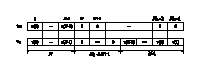
\includegraphics[keepaspectratio, scale=4]
            {parts/FourierAnalysis/imgs/FFT/arbitraryLengthFFT_to_powerOf2_FFT/u2,v2.eps}
            \caption{$u_2,v_2$の構造}
        \end{figure}
        このようにすると$u_2*v_2$の先頭$N$要素が$u*v$と一致する。
        \[ \text{FFT}(u_2*v_2) = \sqrt{N_2}\text{ FFT}(u_2) \text{ FFT}(v_2) \]
        より
        \[ \text{IFFT}(\sqrt{N_2}\text{ FFT}(u_2) \text{ FFT}(v_2)) \]
        により$u_2*v_2$を高速に計算し、結果の先頭$N$要素を切り出せば$u*v$を得る。
        得られた$u*v$の第$k$要素に$\frac{1}{\sqrt{N}} \exp \left(\pi i\frac{-k^2}{N}\right)$を掛ければ$x$のDFTが得られる。
        $v_2$のFFTや$\frac{1}{\sqrt{N}} \exp \left(\pi i\frac{-k^2}{N}\right) \;(k=0,1,\dots,N-1)$は初回の計算結果を保存しておけば別の信号のDFTの計算で再利用できる。


	\part{Laplace変換}
    \chapter{複素指数関数入力に対する伝達関数の作用}
        \begin{shadebox}
            $A>0,\;\omega \in \realNumbers$とする。
            連続時間信号$f: \realNumbers \to \complexNumbers$を次のように定める。
            \[
                f(t) =
                \begin{cases}
                    A\NapierE^{i\omega t} & (t\geq 0) \\
                    0 & (t<0)
                \end{cases}
            \]
            $H: s\in\complexNumbers \mapsto H(s) \in \complexNumbers$をproperで既約な有理関数とする。
            また,$H$の極の実部は全て負であるとする。
            伝達関数が$H(s)$である連続時間システムに信号$f$を入力した時の出力を$g$とすると,十分大きい$t$に対して
            $g(t) \sim H(i\omega)f(t)$となる。
        \end{shadebox}
        \begin{proof}
            \quad\par
            $N_\text{p}$を$H(s)$の分母多項式の相異なる零点の個数とし,それら零点を$p_0,\dots,p_{N_\text{p}}$とする。
            零点$p_k$の次数を$N_{\text{p},k}$とし,$H(s)$の部分分数展開を
            \[ H(s) = c_0 + \sum_{k=1}^{N_\mathrm{p}} \sum_{l=1}^{N_{\mathrm{p},k}} \frac{c_{k,l}}{(s-p_k)^l} \]
            とする。
            ここに$c_0,c_{k,l}\;(k=1,\dots,N_\mathrm{p},l=1,\dots,N_{\mathrm{p},k})$は適当な複素数である。
            $f,g$のLaplace変換をそれぞれ$F,G$とすると$G(s) = H(s)F(s) = A H(s)/(s-i\omega)$である。
            これの部分分数展開に現れる,$1/(s-p_k)^l\;(k=1,\dots,N_\mathrm{p},l=1,\dots,N_{\mathrm{p},k})$に比例する項は逆Laplace変換すると$t^{l-1}\NapierE^{p_k t}$に比例する関数となり,$t\to\infty$で0に収束する。\hfill \rule{10cm}{0.4pt}(1)
            \par
            残りの項,すなわち$1/(s-i\omega)$に比例する項は$AH(i\omega)/(s-i\omega) = H(i\omega)F(s)$となる。
            以上より,十分大きい$t$に対して$g(t) \sim \ILPLC{H(i\omega)F(s)}(t) = H(i\omega)f(t)$となる。
        \end{proof}
        \section{系: 正弦波入力に対する伝達関数の作用}
            \begin{shadebox}
                $A>0,\;\omega \in \realNumbers$とする。
                連続時間信号$f_1,f_2: \realNumbers \to \realNumbers$を次のように定める。
                \[
                    f_1(t) =
                    \begin{cases}
                        A\cos\omega t & (t\geq 0) \\
                        0 & (t<0)
                    \end{cases}
                \]
                \[
                    f_2(t) =
                    \begin{cases}
                        A\sin\omega t & (t\geq 0) \\
                        0 & (t<0)
                    \end{cases}
                \]
                $H$を直前の定理と同じように定める。
                伝達関数が$H(s)$である連続時間\textcolor{red}{実}システムに信号$f_1,f_2$を入力した時の出力をそれぞれ$g_1,g_2$とすると,十分大きい$t$に対して
                \begin{align*}
                    g_1(t) &\sim |H(i\omega)|\cos(\omega t + \Arg\parens*{H(i\omega)}) \\
                    g_2(t) &\sim |H(i\omega)|\sin(\omega t + \Arg\parens*{H(i\omega)})
                \end{align*}
                となる。
            \end{shadebox}
            \begin{proof}
                \quad\par
                $f_1$について示す。
                $f_2$も同様に示せる。
                $f_1(t) = \Re{A\NapierE^{i\omega t}}$であり,実数システムだから出力は$A\NapierE^{i\omega t}$を入力したときの出力の実部と等しい。
                直前の定理の結果を用いて
                \[ g_1(t) = \Re{H(i\omega)A\NapierE^{i\omega t}} = \Re{|H(i\omega)|\NapierE^{i\Arg\parens*{H(i\omega)}}A\NapierE^{i\omega t}} = |H(i\omega)|\cos (\omega t + \Arg\parens*{H(i\omega)}) \]
            \end{proof}
            \begin{proof}
                (直接的な証明)
                \quad\par
                $f_1$について示す。
                $f_2$も同様に示せる。
                直前の定理の証明の(1)までは同じである。
                $f_1,g_1$のLaplace変換をそれぞれ$F_1,G_1$とすると
                \[ F_1(s) = \frac{As}{s^2+\omega^2} = \frac{A}{2}\left(\frac{1}{s+i\omega} + \frac{1}{s-i\omega}\right) \]
                であるから,$G_1(s) = H(s)F(s)$の部分分数展開のうち$1/(s+i\omega),\;1/(s-i\omega)$に比例する項を詳しく調べれば良い。
                $1/(s+i\omega)$の係数は
                \[ \left. G(s)X(s)(s+i\omega) \right|_{s\to-i\omega} = AG(-i\omega)/2\]
                となり,$1/(s-i\omega)$の係数は
                \[ \left. G(s)X(s)(s-i\omega) \right|_{s\to i\omega} = AG(i\omega)/2\]
                となる。
                よってこれらの項の和は
                \begin{align}
                    &\quad \frac{AG(-i\omega)/2}{s+i\omega} + \frac{AG(i\omega)/2}{s-i\omega} = \frac{A}{2}\left(\frac{G(-i\omega)}{s+i\omega} + \frac{G(i\omega)}{s-i\omega}\right) \nonumber\\
                    &= \frac{A}{2}\times\frac{1}{s^2+\omega^2}\left(G(-i\omega)(s-i\omega) + G(i\omega)(s+i\omega)\right) \nonumber\\
                    &= \frac{As}{s^2+\omega^2}\times\frac{1}{2}(G(i\omega)+G(-i\omega)) + \frac{A\omega}{s^2+\omega^2}\times\frac{-1}{2i}(G(i\omega)-G(-i\omega))
                \end{align}
                $G(s)$は有理式なので$G(-i\omega) = \conj{G(i\omega)}$となることに注意して
                \[ \frac{1}{2}(G(i\omega)+G(-i\omega)) = |G(i\omega)|\frac{1}{2}\left(\NapierE^{i\Arg\parens*{G(i\omega)}} + \NapierE^{-i\Arg\parens*{G(i\omega)}}\right) = |G(i\omega)|\cos\Arg\parens*{G(i\omega)} \]
                同様に
                \[ \frac{-1}{2i}(G(i\omega)-G(-i\omega)) = -|G(i\omega)|\sin\Arg\parens*{G(i\omega)} \]
                以上より,
                \begin{align*}
                    (1) &= |G(i\omega)|\left(\cos\Arg\parens*{G(i\omega)}\frac{As}{s^2+\omega^2} - \sin\Arg\parens*{G(i\omega)}\frac{A\omega}{s^2+\omega^2} \right) \\
                    g(t) &\sim \ILPLC{(1)}(t) = |G(i\omega)|\left(\cos\Arg\parens*{G(i\omega)}\cos\omega t - \sin\Arg\parens*{G(i\omega)}\sin\omega t \right) \\
                    &= |G(i\omega)|\cos\left(\omega t + \Arg\parens*{G(i\omega)}\right)
                \end{align*}
            \end{proof}
	\part{Z 変換}
	\chapter{基礎理論}
		\section{逆 Z 変換}
			\label{inv_Z_trans}
			\begin{shadebox}
				$X:\complexNumbers\to\complexNumbers$ は離散時間信号 $x:\integers\to\complexNumbers$ の Z 変換であるとする。
				このとき次式が成り立つ。
				\begin{equation}
					\label{eq:inv_Z_trans}
					x(n) = \frac{1}{2\pi i}\oint_C X(z)z^{n-1}\mathrm{d}z
				\end{equation}
				ここに積分路 $C$ は $X(z)$ のすべての極を含む反時計回りの単純閉曲線である。
			\end{shadebox}
			\begin{proof}
				\begin{align*}
					\frac{1}{2\pi i}\oint_C X(z)z^{n-1}\mathrm{d}z &= \frac{1}{2\pi i}\oint_C \parens*{\sum_{k=-\infty}^\infty x(k)z^{-k}}z^{n-1}\mathrm{d}z \\
					&= \sum_{k=-\infty}^\infty x(k)\frac{1}{2\pi i}\oint_C z^{n-k-1}\mathrm{d}z = \sum_{k=-\infty}^\infty x(k)\delta_{n,k} = x(n)
				\end{align*}
			\end{proof}
		\section{信号とその片側 Z 変換の一対一対応}
			離散時間信号 $x:\integers\to\complexNumbers$ とその片側 Z 変換 $X$ は非負の時間領域について一対一対応する。
			このことは \ref{inv_Z_trans} の証明から明らかである。
			片側 Z 変換の結果に対して式 \eqref{eq:inv_Z_trans} に於いて負の時刻を指定すると,結果は 0 である。
		\section{最終値定理}
			\begin{shadebox}
				$X(z)\;(z\in\complexNumbers)$を離散時間信号$x(n)\;(n \in \integers,\;\forall n<0,x(n)=0)$のZ変換とする。
				$\lim_{n\to\infty} x(n)$が存在するとき次が成り立つ。
				\[ \lim_{z\to1}(z-1)F(z) = \lim_{n\to\infty} x(n) \]
				但し上式に於ける$\lim_{z\to1}$では$z$が実軸上で右側から1に近づくことを意味する。
			\end{shadebox}
			\begin{proof}
				\quad\par
				$\alpha = \lim_{n\to\infty} x(n)$とする。
				発想としては,十分大きい$N\in\naturalNumbers$に対して$\sum_{k=N+1}^\infty x(k)z^{-k} \sim \sum_{k=N+1}^\infty \alpha z^{-k} = \alpha z^{-N}\frac{1}{z-1}$となることを利用する。
				\par
				任意の$\varepsilon \in (0,1)$に対してある$N\in\naturalNumbers$が存在して$\forall n\geq N,\;|x(n)-\alpha|<\varepsilon$となる。
				\begin{align*}
					\quad &\lim_{z\to1}(z-1)F(z) - \alpha = \lim_{z\to1}(z-1)z^N F(z) - \alpha \\
					&= \lim_{z\to1}(z-1)z^N\left(\sum_{k=0}^{N-1} x(k)z^{-k} + \sum_{k=N+1}^\infty x(k)z^{-k}\right) - (z-1)z^N\sum_{k=N+1}^\infty \alpha z^{-k} \\
					&= \lim_{z\to1}(z-1)z^N \sum_{k=N+1}^\infty (x(n) - \alpha)z^{-k} \quad \left(\sum_{k=0}^{N-1}\text{の項は極限で消える}\right) \tag{1} \\
					|(1)| &\leq \lim_{z\to1}(z-1)z^N \sum_{k=N+1}^\infty |x(n) - \alpha|z^{-k} < \lim_{z\to1}(z-1)z^N \sum_{k=N+1}^\infty \varepsilon z^{-k} = \varepsilon
				\end{align*}
			\end{proof}
		\section{複素指数関数入力に対する伝達関数の作用}
			\begin{shadebox}
				$A>0,\;\omega \in \realNumbers$とする。
				離散時間信号$x: \realNumbers \to \complexNumbers$を次のように定める。
				\[
					x(n) =
					\begin{cases}
						Ae^{i\Omega n} & (n\geq 0) \\
						0 & (n<0)
					\end{cases}
				\]
				$H: z\in\complexNumbers \mapsto H(z) \in \complexNumbers$を,$1/z$を変数とした有理式として既約であるような有理関数とする。
				また,$H$の極の絶対値は全て1未満であるとする。
				伝達関数が$H(z)$である離散時間システムに信号$x$を入力した時の出力を$y$とすると,十分大きい$n$に対して
				$y(n) \sim H(\NapierE^{i\Omega})x(n)$となる。
			\end{shadebox}
			\begin{proof}
				\quad\par
				$N_\text{p}$を$H(s)$の相異なる極の個数とし,それら極を$p_0,\dots,p_{N_\text{p}}$とする。
				極$p_k$の次数を$N_{\text{p},k}$とし,$H(z)$の部分分数展開を
				\[ H(z) = c_0 + \sum_{k=1}^{N_\mathrm{p}} \sum_{l=1}^{N_{\mathrm{p},k}} \frac{c_{k,l}}{(1-p_kz^{-1})^l} \]
				とする。
				ここに$c_0,c_{k,l}\;(k=1,\dots,N_\mathrm{p},l=1,\dots,N_{\mathrm{p},k})$は適当な複素数である。
				$x,y$のZ変換をそれぞれ$X,Y$とすると$Y(z) = H(z)F(z) = A H(z)/(1-\NapierE^{i\Omega}z^{-1})$である。
				これの部分分数展開に現れる,$1/(1-p_k z^{-1})^l\;(k=1,\dots,N_\mathrm{p},l=1,\dots,N_{\mathrm{p},k})$に比例する項は逆Z変換すると$n$の多項式と公比$p_k$の等比級数の積となり,$n\to\infty$で0に収束する。
				(このことはZ変換の性質: 時間シフト$\mathcal{Z}[x(n+k)] = z^kX(z)$,およびZ領域微分$\mathcal{Z}[nx(n)] = -z\derivLong{\mathcal{Z}[x(n)]}{z}{}$を繰り返し用いることで分かる)
				\par
				残りの項,すなわち$1/(1-\NapierE^{i\Omega}z^{-1})$に比例する項は$AH(\NapierE^{i\Omega})/(1-\NapierE^{i\Omega}z^{-1}) = H(\NapierE^{i\Omega})X(z)$となる。
			\end{proof}
	% \chapter{IIRフィルタの計算手順}
	% 	\begin{figure}[H]
	% 		\centering
	% 		\includegraphics[keepaspectratio, scale=5]
	% 		{\currfiledir/figs/IIR-filter/calculationMethod/blockDiagram.pdf}
	% 		\caption{IIRフィルタのブロック図の例}
	% 	\end{figure}
	% 	上の例で示したIIRフィルタの出力は以下の手続きで計算できる(仕事で関わっていたデジタル無線機の信号処理部でそうやっていた)。
	% 	\begin{enumerate}
	% 		\item $D_1,\cdots D_4 \leftarrow 0$
	% 		\item $n \leftarrow 0$
	% 		\item $\alpha \leftarrow a_1D_1 + \cdots a_4D_4$
	% 		\item $\beta \leftarrow b_1D_1 + \cdots b_4D_4$
	% 		\item $\gamma \leftarrow x(n) + \beta$
	% 		\item $y(n) \leftarrow \alpha + a_0\gamma$
	% 		\item $D_4 \leftarrow D_3,\;D_3 \leftarrow D_2,\;D_2 \leftarrow D_1,\;D_1 \leftarrow \gamma$
	% 		\item $n \leftarrow n+1$
	% 		\item $n$が$x$の定義域の末尾に達しているなら終了。そうでないなら3に戻る。
	% 	\end{enumerate}
	\part{フィルタ}
    \chapter{離散時間フィルタ}
    離散時間フィルタは次の通り分類される。
    \begin{enumerate}
        \item feedforward フィルタ\\
        出力がそれ以前の出力に依存しない。ディジタル計算機で実現するため,インパルス応答の長さは有限であると約束する。
        \item feedback フィルタ\\
        出力がそれ以前の出力に依存する。実用上の意味のあるフィルタは多くの場合 feedforward 構造を含み,そこに入力信号が入る。
        インパルス応答の長さは無限である場合が多いが,有限の場合もある(例えば CIC フィルタ)。
    \end{enumerate}
    \section{連続時間系のフィルタ処理を離散時間系で観測したときの振る舞い}
    ここでは,連続時間系でフィルタ処理を行った結果を離散時間系で観測したときの振る舞いを考える。
    この問題は実用上興味深い。
    物理系の状態をセンサでコンピュータに取り込み,有益な計算をする状況がこれに当てはまる。
    具体的には,無線受信機の直交分離出力であるIQ信号(連続時間信号)をADCで一定周期でサンプリングしてCPUに取り込んで復調の計算を行う状況が考えられる。
    \begin{shadebox}
        $h:\realNumbers\to\realNumbers$を連続時間信号とする。
        $H:\complexNumbers\to\complexNumbers$を$h$のLaplace変換とする。
        インパルス応答が$h$である連続時間フィルタを連続時間系の複素正弦波信号$x(t) = A\exp i(\omega_0 t + \phi)\;(A>0,\omega_0,\phi\in\realNumbers)$に適用した出力を$y=h*x$とする。
        $x,y$をサンプリング周期$\Ts$でサンプリングした離散時間信号を$\xd: n\in\integers\mapsto x(n\Ts), \yd: n\in\integers\mapsto y(n\Ts)$とする。
        このとき次式が成り立つ。
        \[ \DTFTwithArg{\yd}{\bm{\omega}} = H(i\omega_0)\DTFTwithArg{\xd}{\bm{\omega}} \]
    \end{shadebox}
    \begin{proof}
        \begin{align*}
            \DTFTwithArg{\yd}{\bm{\omega}} &= \sum_{m=-\infty}^\infty y(n\Ts)\exp \left(-i n\Ts\omega\right) = \sum_{m=-\infty}^\infty (h*x)(n\Ts)\exp \left(-i n\Ts\omega\right) \\
            &= \sum_{m=-\infty}^\infty \left(\integrate{-\infty}{\infty}{h(\tau)x(n\Ts-\tau)}{}{\tau}\right)\exp \left(-i n\Ts\omega\right) \\
            &= \integrate{-\infty}{\infty}{h(\tau)\sum_{m=-\infty}^\infty x(n\Ts-\tau)\exp \left(-i n\Ts\omega\right)}{}{\tau} \\
            &= \integrate{-\infty}{\infty}{h(\tau)\sum_{m=-\infty}^\infty A\exp i(\omega_0 (n\Ts-\tau) + \phi)\exp \left(-i n\Ts\omega\right)}{}{\tau} \\
            &= \integrate{-\infty}{\infty}{h(\tau) \exp(-i\omega_0\tau)\sum_{m=-\infty}^\infty A\exp i(\omega_0 n\Ts + \phi)\exp \left(-i n\Ts\omega\right)}{}{\tau} \\
            &= \DTFTwithArg{\xd}{\omega} \integrate{-\infty}{\infty}{h(\tau) \exp(-i\omega_0\tau)}{}{\tau} = \DTFTwithArg{\xd}{\omega}H(i\omega_0)
        \end{align*}
    \end{proof}
    \section{feedback フィルタの出力値の範囲}
    \newcommand{\Nff}{{N_{\text{ff}}}}
    \newcommand{\Nfb}{{N_{\text{fb}}}}
    \newcommand{\hInit}[1]{{h_{\text{init},#1}}}
    \newcommand{\Minit}[1]{{M_{\text{init},#1}}}
    feedback フィルタの入力の絶対値が制限されるときの出力の絶対値の最大値を求める。
    この関係は feedback フィルタを実装する際に,内部の記憶素子と演算素子に必要なビット幅を決める際に役立つ。
    ここでは拡張性を重視して信号の終域を $\complexNumbers$ としているが,用途に応じて $\realNumbers$ に制限してもよい。
    \begin{shadebox}
        F を feedback フィルタとし,$x,\;y:\integers\to\complexNumbers$ をそれぞれ入力と出力とする。
        $x$ の絶対値が $M_x(\geq 0)$ 以下であるとする。
        F の漸化式が次式であるとする。
        \[ y(n) = \sum_{k=0}^\Nff a_k x(n-k) - \sum_{l=1}^\Nfb b_l y(n-l) \]
        ここに $\Nff,\;\Nfb\in\naturalNumbers$ はそれぞれ feedforward 経路、feedback 経路のタップ数であり, $a_k,\;b_l\in\complexNumbers$ は係数である。
        \par
        $h:\integers\to\complexNumbers$ を F のインパルス応答とし,$\hInit{m}:\integers\to\complexNumbers$ を次式の逆 Z 変換とする。
        \[ \frac{\sum_{\tilde{l}=m}^\Nfb b_{\tilde{l}} z^{-(\tilde{l}-m)}}{1+\sum_{l=1}^\Nfb b_l z^{-l}} \]
        $\Minit{m}\coloneq\max_n {\abs{\hInit{m}(n)}}$ とする。
        $y$ の値の範囲について次式が成り立つ。
        \[ \max_{n\in\naturalNumbers\cup\{0\}}\abs{y(n)} \leq M_x\sum_{k=0}^\infty\abs{h(k)} + \sum_{l=1}^\Nfb\abs{y(-l)}\Minit{m} \]
        とくに,負の時刻について $y$ の値が 0 であるならば次式が成り立つ。
        \[ \max_{n\in\naturalNumbers\cup\{0\}}\abs{y(n)} \leq M_x\sum_{k=0}^\infty\abs{h(k)} \]
    \end{shadebox}
    \begin{proof}
        % TODO: Write this.
    \end{proof}
    \input{\currfiledir/sections/feedforward_filter_design.tex}
    \section{CIC up-sampler}
    \label{CIC up-sampler}
    \newcommand{\XNAF}{X_\text{NAF}}
    \newcommand{\YNAF}{Y_\text{NAF}}
    \newcommand{\tYNAF}{\tilde{Y}_\text{NAF}}
    \newcommand{\XNF}{X_\text{NF}}
    \newcommand{\YNF}{Y_\text{NF}}
    \newcommand{\tYNF}{\tilde{Y}_\text{NF}}

    $R$ はアップ・サンプリング・レートを表し、$N$ は差分器と積算器それぞれの段数を表す。
    \par
    FPGA, ASIC による実装を前提として加算器(組み合わせ論理回路)の直後に Flip-flop を置く。
    Web 情報の多くはこれによる遅延を考慮しておらず、本書の結果と異なる数式を導いているが、影響があるのは遅延量だけであり、本質は変わらない。
    \subsection{周波数スペクトラム}
        \label{CIC up-sampler の周波数スペクトラム}
        差分器 1 つの漸化式は $y(n) = x(n-1) - x(n-2)$ であり、伝達関数は $(z^{-1})(1-z^{-1})$ である。
        ここに $x,y:\integers\to\complexNumbers$ は差分器への入力と出力である。
        同様に記号を流用して積算器の入出力 1 つの漸化式は $y(n) = y(n-1) + x(n-1)$ であり、伝達関数は $(z^{-1})/(1-z^{-1})$ である。
        Noble Identity を用いて $R$ 倍オーバー・サンプラを最前段に移動させると、 $R$ 倍オーバー・サンプラの後ろの伝達関数は次式である。
        \[ H_\text{C,I}(z) = z^{-N(R+1)}\parens*{\frac{1-z^{-R}}{1-z^{-1}}}^N = z^{-N(R+1)}\parens*{\sum_{n=0}^{R-1} z^{-n}}^N \]
        これは、長さ $R$ の区間の和をとるブロックを $N$ 段従属接続して $N(R+1)$ だけ遅延させる操作と等価である。
        この系に対して $R$ 倍にオーバー・サンプルした結果を入力して得られる出力が CIC up-sampler の出力である。
        \par
        CIC up-sampler の出力の絶対値が最大となるのは、入力のビット幅が許す範囲の絶対値最大(この値を $x_\text{MAX}$ とおく)の定数列が入力された場合であり、値は次式である。
        \begin{equation}
            x_\text{MAX}R^{N-1}
            \label{equation:CIC up-sampler の出力の絶対値の最大値}
        \end{equation}
        このことから直ちに解るが、 CIC up-sampler の直流ゲインは $R^{N-1}$ である。
        \par
        入力と出力の DTFT をそれぞれ $\XNAF(\Omega), \YNAF(\Omega)$ ($\Omega$ は正規化角周波数) とする。
        $H_\text{C,I}(z)$ に於いて $z = \exp(-i\Omega)$ とし、\ref{オーバー・サンプリングされた信号の DTFT} を適用し、周波数スペクトラムとして次式を得る。
        \begin{align*}
            \YNAF(\Omega) &= \exp(-iN(R+1)\Omega)\frac{\parens*{1-\exp\parens*{-iR\Omega}}^N}{R\parens*{1-\exp\parens*{-i\Omega}}^N}\XNAF(R\Omega) \\
            &= \exp\parens*{-i\frac{\Omega}{2}N(3R+1)}\parens*{\frac{\sin(R\Omega/2)}{\sin(\Omega/2)}}^N \XNAF(R\Omega)
        \end{align*}
        % ↓ 間違い。Noble Identity を用いて移動したオーバー・サンプラが区間和の 1 つと相殺することから勘違いした。ゲインが相殺するとはいえ、レートは元に戻らないのだから、完全に無視した式になるはずがない。
        % \begin{align*}
        %     \YNAF(\Omega) &= \exp(-iN(R+1)\Omega)\frac{\parens*{1-\exp\parens*{-iR\Omega}}^{N-1}}{\parens*{1-\exp\parens*{-i\Omega}}^{N-1}}\XNAF(R\Omega) \\
        %     &= \exp\parens*{-iN(R+1)\Omega}\exp\parens*{-i\frac{\Omega}{2}(N-1)(R-1)}\parens*{\frac{\sin(R\Omega/2)}{\sin(\Omega/2)}}^{N-1} \XNAF(R\Omega) \\
        %     &= \exp\exp\parens*{-i\frac{\Omega}{2}N(3R+1)}\parens*{\frac{\sin(R\Omega/2)}{\sin(\Omega/2)}}^{N-1} \XNAF(R\Omega)
        % \end{align*}
        正規化周波数で表現しなおして $\XNF(F) = \XNAF(2\pi F), \YNF(F) = \YNAF(2\pi F)$ とすれば次式を得る。
        \begin{align}
            \YNF(F) &= \exp\parens*{-i\frac{2\pi F}{2}N(R-1)}\parens*{\frac{\sin(R 2\pi F/2)}{\sin(2\pi F/2)}}^N \XNF(R F) \nonumber \\
            &= \exp\parens*{-i\pi N(3R+1)F}\parens*{\frac{\sin(\pi R F)}{\sin(\pi F)}}^N \XNF(R F) \label{equation:CIC up-sampler の周波数スペクトラム}
        \end{align}
        この式は $F\to 0$の極限で $R^N \XNF(0)$ となる。
        しかし入力を直流としたときに出力の絶対値が $R^N$ 倍になるわけではない。
        なぜならば既に述べたように、 Noble Identity を用いて移動したオーバー・サンプラが、伝達関数に含まれる長さ $R$ の区間和の 1 つと相殺するからである。
        周波数スペクトラムと「振幅特性」(すぐ後に明かされるように、この単語は正しく定義されないので敢えて「」付きで示した)が一致しない原因は単純で、オーバー・サンプルという非線形な操作を加えた結果、正弦波入力に対する出力が正弦波とならないからである。
        この状況では「振幅特性」自体が定義できない。
        アップ・サンプルによって正弦波が緻密になって出力されたように見えても、それは「そう見える」だけであり、厳密には正弦波ではなく広がりをもったスペクトラムをもつ信号に変わっている。
    \subsection{差分器と積算器に必要なビット幅}
        \subsubsection{差分器のビット幅}
            差分器の出力の絶対値が最大となるのは、入力のビット幅が許す範囲の最大振幅の交代列が入力された場合である。
            よって、差分器の出力のビット幅は入力のそれの 2 倍を確保すればよく、$N$ 段目の差分器の出力のビット幅は初段の入力のビット幅 + $N$ とすればよい。
        \subsubsection{積算器のビット幅(解析的な方法)}
            CIC up-sampler の入力のビット幅を $B$ とする。
            まず、\cref{equation:CIC up-sampler の出力の絶対値の最大値} より最終段の積算器(第 $N$ 積算器)の出力のビット幅は $B + (N-1)\log_2 R$ を確保すれば必要十分である。
            \par
            最終段より前の積算器については必要十分なビット幅を解析的に求めることはできないが、十分な値であれば次のようにして求められる。
            \par
            第 $(N-1)$ 積算器の出力のビット幅を考える。
            第 $2$ 差分器から第 $(N-1)$ 積算器までに注目すると、これはステージ数 $N-1$ の CIC up-sampler となっている。
            このことと、元の第 $1$ 差分器の出力の絶対値の最大値がビット幅 $B+1$ で収容できることから、第 $(N-1)$ 積算器の出力はビット幅 $B + 1 + (N-2)\log_2 R$ を確保すれば十分である。
            (元の第 $1$ 差分器の出力が最大値で一定していることはあり得ないことは容易に解る。
            この点を無視して上限で評価しており、故に「必要な」ビット幅からの乖離がある。)
            \par
            同様にして次々に内側の小さい CIC up-sampler を考えてゆくと、十分なビット幅が求まる。
        \subsubsection{積算器のビット幅(数値的な方法)}
            最終段については既に述べたように解析的に求められるのでここでは扱わない。
            \par
            Noble Identity を用いて $R$ 倍オーバー・サンプラを最前段に移動した後、第 1 差分器から第 $n\in\{1,2,...,N-1\}$ 段の積算器までの部分系の伝達関数を考えると次式を得る。
            \[ \frac{(1-z^{-R})^N}{(1-z^{-1})^n} = (1-z^{-R})^{N-n}\parens*{\sum_{n=0}^{R-1} z^{-n}}^n \]
            上式のうち、$\sum_{n=0}^{R-1} z^{-n}$ 1つ分については、この系の前段に移動された $R$ 倍オーバー・サンプラと相殺し、ビット幅増加に寄与しない。
            よって、ビット幅の増加に寄与する部分は次式である。
            \begin{equation}
                \frac{(1-z^{-R})^N}{(1-z^{-1})^n} = (1-z^{-R})^{N-n}\parens*{\sum_{n=0}^{R-1} z^{-n}}^{n-1} \label{equation:CIC up-sampler の部分系の伝達関数}
            \end{equation}
            これは抽出された部分系の有限インパルス応答の z 変換である。
            この系の応答の絶対値が最大となるような作為的な入力に対する応答を収容できるビット幅を確保すればよい。
            そのような最悪の応答は \cref{equation:CIC up-sampler の部分系の伝達関数} を計算機代数システムを用いて $z^{-1}$ の多項式として展開し、係数の絶対値の総和をとることで得られる。
    \subsection{CIC up-sampler 補償フィルタ}
        \newcommand{\HCNF}{H_\text{C,NF}}

        \cref{equation:CIC up-sampler の周波数スペクトラム} より、アップ・サンプリングにより $\XNF$ には $F$ に依存する因子が掛かる。
        これをできるだけ補正するために、CIC up-sampler の直前で前記の因子の逆特性を近似する畳み込み型 FIR フィルタ(以下単に「FIR フィルタ」と呼ぶ)の適用を考える($F$ に依存しないスケーリング因子 $1/R$ は容易に補正できるので、今は無視する)。
        このフィルタの周波数スペクトラムを $\HCNF$ とすると次式が成り立つ。
        \[ \YNF(F) = \exp\parens*{-i\pi N(3R+1)F}\parens*{\frac{\sin(\pi R F)}{\sin(\pi F)}}^N \HCNF(R F)\XNF(R F) \]
        $\HCNF(F)$ に求められるのは $F \in [-1/2,1/2]$ の範囲で次式を近似することである。
        \begin{equation}
            \exp\parens*{i\pi N\frac{R-1}{R}F}\parens*{\frac{\sin(\pi F/R)}{\sin(\pi F)}}^N \label{equation:CIC up-sampler 補償フィルタの理想的な周波数スペクトラム}
        \end{equation}
        $R$ が大きいとき、$\sin(\pi F/R) \sim \pi F/R$ として \cref{equation:CIC up-sampler 補償フィルタの理想的な周波数スペクトラム} の振幅特性が(Fに依存しないスケールの違いを除いて) $1/\sinc(\pi F)^N$ に漸近する。
        \par
        $\HCNF$ が周期 1 の関数であることから、 $[-1/2,1/2]$ の区間全体で上式を近似することはできない(端点で微分不可能になる)。
        現実には、$\alpha[-1/2,1/2]\;(0<\alpha<1)$ の範囲を Remez のアルゴリズム等で近似する。
        $\alpha$ が 1 に近づく程、必要な係数が増える。
        \cref{equation:CIC up-sampler の周波数スペクトラム} が示すように CIC up-sampler の位相特性が線形なので Remez のアルゴリズムでは振幅の補正だけを気にして係数設計してよい(生成される畳み込み型 FIR フィルタ(以下単に「FIR フィルタ」と呼ぶ)の位相特性も線形なので合成系の位相特性も線形となる)。
        \par
        アップ・サンプリングを全て CIC up-sampler で行うのではなく、一部を CIC up-sampler の前段のゼロ埋めと FIR フィルタ(「FIR フィルタ 1」と呼ぶ)に分担させ、そのフィルタに後段の CIC up-sampler の補正フィルタを兼任させる(合成する)こともしばしば行われる。
        例えば、 FIR フィルタ 1 の直前で x2 zero-padding を行う場合、フィルタ 1 では $0.8\times[-1/4,1/4]$ の領域で \cref{equation:CIC up-sampler 補償フィルタの理想的な周波数スペクトラム} を近似し、$[-1/2,-1/2+0.8/4]\cup[1/2-0.8/4,1/2]$ の領域を阻止帯とするように Remez のアルゴリズムで係数を計算する。
\section{CIC down-sampler}
    $R$ はダウン・サンプリング・レートを表し、$N$ は差分器と積算器それぞれの段数を表す。
    \ref{CIC up-sampler} と同様に加算器(組み合わせ論理回路)の直後に Flip-flop を置く。
    \subsection{周波数スペクトラム}
        Noble Identity を用いて $R$ 倍アンダー・サンプラを最終段に移動させると、\ref{CIC up-sampler の周波数スペクトラム} と同様にして、 $1/R$ 倍アンダー・サンプラより前の伝達関数は次式である。
        \[ H_\text{I,C}(z) = z^{-N(R+1)}\parens*{\frac{1-z^{-R}}{1-z^{-1}}}^N = z^{-N(R+1)}\parens*{\sum_{n=0}^{R-1}z^{-n}}^N \]
        これは、長さ $R$ の区間の和をとるブロックを $N$ 段従属接続して $N(R+1)$ だけ遅延させる操作と等価である。
        この系の出力を 1/R でサンプリングした結果が CIC down-sampler の出力である。
        よって、系の出力の絶対値が最大となるのは、絶対値が最大の定数 ($x_\text{MAX}$ とする)を入力し続けたときであり、そのときの出力の絶対値は $R^N x_\text{MAX}$ である。
        このことから直ちに解るが、直流ゲインは $R^N$ である。
        \par
        入力の DTFT を $\XNAF(\Omega)$ ($\Omega$ は正規化角周波数) とする。
        $1/R$ 倍アンダー・サンプラより前の出力の DTFT を $\tYNAF(\Omega)$ とする。
        $H_\text{I,C}(z)$ に於いて $z = \exp(-i\Omega)$ とすると次式が成り立つ。
        \begin{align*}
            \tYNAF(\Omega) &= \exp(-iN(R+1)\Omega)\frac{\parens*{1-\exp\parens*{-iR\Omega}}^N}{\parens*{1-\exp\parens*{-i\Omega}}^N}\XNAF(\Omega) \\
            &= \exp\parens*{-i\frac{\Omega}{2}N(3R+1)}\parens*{\frac{\sin(R\Omega/2)}{\sin(\Omega/2)}}^N \XNAF(\Omega)
        \end{align*}
        正規化周波数で表現しなおして $\XNF(F) = X(2\pi F), \tYNF(F) = \tYNAF(2\pi F)$ とすれば次式を得る。
        \[ \tYNF(F) = \exp\parens*{-i\pi N(3R+1)F}\parens*{\frac{\sin(\pi R F)}{\sin(\pi F)}}^N \XNF(F) \]
        これと \ref{アンダー・サンプリングされた信号の DTFT} より、$1/R$ 倍アンダー・サンプラの出力を正規化周波数で表現した周波数スペクトラムは次式である。
        \begin{align}
            \YNF(F) &= \frac{1}{R}\sum_{n=0}^{R-1} \tYNF((F-n)/R) \nonumber \\
            &= \frac{1}{R}\sum_{n=0}^{R-1} \exp\parens*{-i\pi N(F-n)(3R+1)/R}\parens*{\frac{\sin(\pi(F-n))}{\sin(\pi(F-n)/R)}}^N \XNF((F-n)/R) \label{equation:CIC down-sampler の周波数スペクトラム}
        \end{align}
        \ref{アンダー・サンプリングされた信号の DTFT} でも述べられているが、全体に掛けられている $1/R$ は DTFT の内積計算の対象となる点の数が $1/R$ に減ったことに由来しており、振幅が $1/R$ になるわけではない。
    \subsection{差分器と積算器に必要なビット幅}
        入力は固定小数点数であるが、全体を適当に2のべき乗倍したものとして見直して符号付整数として扱っても系としては等価なので、以後そうする。
        入力側(サンプル・レートが高い側)から入力される符号付整数のビット幅を $B$ とする。
        \par
        先の議論から、最終段の出力のビット幅は $\ceil{1 + \log_2\parens{R^N 2^{B-1}}} = B + \ceil{N\log_2 R}$ あれば十分であることが判る。
        \par
        積算器はオーバー・フローし得るが、溢れた桁を捨てる操作が modulo 演算であることと、最終段の出力のビット幅を考えれば、最終段より左側の全ての段のビット幅を最終段と等しくしておけば問題ない(無限のビット幅を持つ仮想的な系と同じ出力が得られる)ことが判る。
    \subsection{CIC down-sampler 補償フィルタ}
        \cref{equation:CIC down-sampler の周波数スペクトラム} より、ダウン・サンプリングにより $\XNF$ には $F$ に依存する因子が掛かる。
        これをできるだけ補正するために、CIC down-sampler の直後で前記の因子の逆特性を近似する畳み込み型 FIR フィルタの適用を考える($F$ に依存しないスケーリング因子 $1/R$ は容易に補正できるので、今は無視する)。
        ダウン・サンプリング後に補償用フィルタを掛けるので第 1 Nyquist 領域のみに関心を払えばよい(とうより、それを超えてできることはない)。
        第 1 Nyquist 領域のみを抽出し、補償用フィルタの周波数スペクトラムを $\HCNF$ とすると次式が成り立つ。
        \[ \YNF(F) = \HCNF(F) \frac{1}{R} \exp\parens*{-i\pi N F(3R+1)/R}\parens*{\frac{\sin(\pi F)}{\sin(\pi F/R)}}^N \XNF(F/R) \]
        $\HCNF(F)$ に求められるのは $F \in [-1/2,1/2]$ の範囲で次式を近似することである。
        \begin{equation}
            \exp\parens*{i\pi N F(3R+1)/R}\parens*{\frac{\sin(\pi F/R)}{\sin(\pi F)}}^N
        \end{equation}
        この式は偏角の差を除いて \cref{equation:CIC up-sampler 補償フィルタの理想的な周波数スペクトラム} と一致するため、補償用フィルタの設計手法は CIC up-sampler 補償フィルタと同じものを適用できる。



	\part{周波数変換}
    \chapter{ヘテロダイン}
    元の信号が実数値か複素数値か、変換後の出力を複素数値のまま扱えるのか、それとも実数しか扱えないのか、状況設定次第で何通りも考えられるが、ここでは登場頻度が高いケースについて記す。
    \section{連続時間複素数値信号を上方変換して実数値信号を送信し、受信側で複素数値信号を復元する}
        無線通信で使われる手法である。
        \subsection{計算}
            $I_0, Q_0:\realNumbers\to\realNumbers,\;x_0:\realNumbers\to\complexNumbers; t\in\realNumbers\mapsto I_0(t) + iQ_0(t),\;\omega > 0$ とする。
            $x_0$ は所謂ベースバンド信号である。
            送信側は次式で上方変換された信号を $x_1$ 作る。
            \[ x_1(t) = x(t)\exp(i\omega t) = I_0(t)\cos\omega t - Q_0(t)\sin\omega t + i\parens*{Q_0(t)\cos\omega t + I_0(t)\sin\omega t} \]
            無線通信に於いては $x_1$ の実部が送信される。
            受信側では次式で下方変換された信号 $x_2$ を得る。
            \begin{align*}
                x_2(t) &= \Re{x_1(t)}\exp(-i\omega t) \\
                &= \frac{1}{2}\bracks*{I_0(t)(1+\cos 2\omega t) + Q_0(t)\sin 2\omega t - i(I_0(t)\sin 2\omega t - Q_0(t)(1-\cos 2\omega t))}
            \end{align*}
            これにLPFを掛けて $2\omega t$ で振動する成分を除去して次の信号を得る。
            \[ x_3(t) \coloneq \frac{1}{2}(I_0(t) + iQ_0(t)) \]
        \subsection{サイドバンドの考察}
            送信された $\Re{x_1}$ は実時間信号だからスペクトラムは偶関数である。
            前述の受信側の操作ではスペクトラムの右半分を原点に向かって $\omega$ だけ平行移動させ、LPFで高周波を消している。


	\part{離散時間化}
    \chapter{0次ホールド}
    \providecommand{\FT}[1]{\mathcal{F}\parens*{#1}}
    \providecommand{\Ts}{T_\text{s}}
    \section{0次ホールドされた離散時間信号の周波数特性}
        \label{0次ホールドされた離散時間信号の周波数特性}
        \subsection{動機}
            離散時間信号を仮に量子化誤差なくDA変換できた場合の周波数スペクトラムを計算したい。
        \subsection{主張}
            $\xd:\integers\to\complexNumbers$ を離散時間信号とする。
            $\Xd$ を $\xd$ のDTFTとする。
            $\Ts>0$ をサンプル周期として $\xd$ の0次ホールドで生成した階段状の連続時間信号を $x$ とする。
            $u:\realNumbers\to\braces{0,1}$ を幅 $\Ts$ のパルスとする。
            \[
                u(t) = \begin{cases}
                    1 & 0\leq t < \Ts \\
                    0 & \text{otherwise}
                \end{cases}
            \]
            $x$ は次式で表される。
            \[ x(t) = \sum_{n=-\infty}^\infty \xd(n)u(t-n\Ts) \]
            次の図は $\Ts=1,\xd(n) = \sin\parens{2\pi n/12}\;(0\leq n\leq 24),\;\xd(n) = 0\;(n<0,24<n)$ の例である。
            \begin{figure}[H]
                \centering
                \includegraphics[keepaspectratio, scale=0.8]
                {\currfiledir/figs/x1.pdf}
                \caption{$x$の例}
                \label{figure:離散時間信号のDAC出力の例}
            \end{figure}
            以上の下、 $x$ のFourier変換 $X$ は次式である。
            \[ X(\omega) = \frac{\Ts}{\sqrt{2\pi}}\exp\parens*{-i\frac{\Ts}{2}\omega}\parens*{\sinc \frac{\Ts}{2}\omega}\Xd(\omega) \]
            $\Xd(\omega)$ が $2\pi/\Ts$ 周期関数であることに注意すれば、$\Xd(\omega)$ の第1 Nyquist領域の形状が位相回転 $\exp\parens{-i \omega n\Ts}$ とレベル減衰 $\sinc\omega\Ts/2$ を伴いつつ周期的に無限に繰り返されていることがわかる。
            次の図は\ref{figure:離散時間信号のDAC出力の例}に対応する $X$ の例である。
            \begin{figure}[H]
                \centering
                \includegraphics[keepaspectratio, scale=0.8]
                {\currfiledir/figs/FT_of_x1.pdf}
                \caption{$X$の例。横軸は正規化角周波数}
            \end{figure}
        \subsection{導出}
            \begin{proof}
                \quad\par
                \[ X(\omega) = \FT{\sum_{n=-\infty}^\infty \xd(n)u(t-n\Ts)}(\omega) = \sum_{n=-\infty}^\infty \xd(n)\FT{u(t-n\Ts)}(\omega) \tag{1} \]
                ここで次式が成り立つ。
                \begin{align*}
                    \FT{u(t-n\Ts)}(\omega) &= \exp\parens*{-i \omega n\Ts}\FT{u}(\omega) = \exp\parens*{-i \omega n\Ts}\frac{1}{\sqrt{2\pi}}\integrate{0}{\Ts}{\exp\parens*{-i\omega t}}{}{t} \\
                    &= \frac{i}{\omega\sqrt{2\pi}}\parens*{\exp\parens*{-i \omega\Ts}-1}\exp\parens*{-i \omega n\Ts} \\
                    &= \frac{i}{\omega\sqrt{2\pi}}\exp\parens{-i \omega n\Ts}\exp\parens{-i \omega\Ts/2}\parens*{\exp\parens*{-i \omega\Ts/2} - \exp\parens*{i \omega\Ts/2}} \\
                    &= \frac{i}{\omega\sqrt{2\pi}}\exp\parens{-i \omega n\Ts}\exp\parens{-i \omega\Ts/2}(-2i)\sin\frac{\omega\Ts}{2} \\
                    &= \frac{2}{\omega\sqrt{2\pi}}\exp\parens{-i \omega n\Ts}\exp\parens{-i \omega\Ts/2}\sin\frac{\omega\Ts}{2} \\
                    &= \frac{\Ts}{\sqrt{2\pi}}\exp\parens{-i \omega n\Ts}\exp\parens{-i \omega\Ts/2}\sinc\frac{\omega\Ts}{2}
                \end{align*}
                これを式(1)に適用して次式を得る。
                \begin{align*}
                    X(\omega) &= \sum_{n=-\infty}^\infty \xd(n)\frac{\Ts}{\sqrt{2\pi}}\exp\parens{-i \omega n\Ts}\exp\parens{-i \omega\Ts/2}\sinc\frac{\omega\Ts}{2} \\
                    &= \frac{\Ts}{\sqrt{2\pi}}\exp\parens{-i \omega\Ts/2}\sinc\frac{\omega\Ts}{2} \sum_{n=-\infty}^\infty \xd(n)\exp\parens{-i \omega n\Ts} \\
                    &= \frac{\Ts}{\sqrt{2\pi}}\exp\parens*{-i\frac{\Ts}{2}\omega}\parens*{\sinc \frac{\Ts}{2}\omega}\Xd(\omega)
                \end{align*}
            \end{proof}
    \section{inverse-sinc-filter}
        \subsection{背景}
            離散時間信号をDA変換した結果のFourier変換には次式で表される変化が積の形で含まれることを\ref{0次ホールドされた離散時間信号の周波数特性}で述べた。
            \[ \sinc \frac{\Ts}{2}\omega = \sinc \frac{\Omega}{2} \]
            ここに $\Ts$ はサンプリング周期, $\Omega$ は正規化角周波数である。
            変化の中には上式の他に $\exp\parens*{-i\frac{\Ts}{2}\omega}$ という項も含まれるが、これは一定の群遅延が加わる(線形位相特性)だけであり、実用上無害なので無視する。
            次の図は $\abs{\sinc \frac{\Omega}{2}}$ をプロットしたものである。
            \begin{figure}[H]
                \centering
                \includegraphics[keepaspectratio, scale=0.6]
                {\currfiledir/figs/sinc-shaped_gain_distortion_with_ideal_DA.pdf}
                \caption{量子化誤差のないDA変換結果の sinc 状ゲイン歪み}
            \end{figure}
            上の図から、第1 Nyquist 領域の端 $-\pi, \pi$ で約 -3dB のゲイン低下が生じていることが解る。
            実は0次ホールドで出力する直前に、上手く設計された10タップ程度の畳み込み型 FIR フィルタを掛けてこの影響を緩和し、下図のようなゲイン特性に変更できる。
            このフィルタは「inverse-sinc フィルタ」と呼ばれる。
            \begin{figure}[H]
                \centering
                \includegraphics[keepaspectratio, scale=0.6]
                {\currfiledir/figs/mitigated_distortion_with_inverse-sinc_filter.pdf}
                \caption{inverse-sinc フィルタによって緩和されたゲイン歪み(凡例の3つ目の曲線)}
                \label{inverse-sinc フィルタによって緩和されたゲイン歪み}
            \end{figure}
            inverse-sinc フィルタは $[-\pi, \pi]$ で sinc 状歪みの逆特性を近似するフィルタである。
            DA変換の対象とする信号は通常、サンプリング定理を念頭に置いてスペクトラムが $[-\pi,\pi]$ の領域に収まる信号であるから、上述の補正が十分に機能する。
            以下ではこのフィルタの設計方法の1つを述べる。
        \subsection{係数の導出}
            大雑把に言えば、フィルタ係数に対応する DTFT が $[-\pi,\pi]$ で $1/\sinc(\Omega/2)$ を近似するように最小二乗法で係数を決定する。
            \par
            フィルタ係数 $a:\integers\to\realNumbers$ は偶対称な実数値関数とし、非零の係数の個数を奇数とする。
            数式で述べれば $N\in\naturalNumbers,\;\forall n\in\integers\;a(-n) = a(n),\forall n>N\;a(n) = 0$ である。
            この制約条件が唯一の方法ではないだろうが、後に見るようにこれで十分な性能を得られる。
            \par
            $a$ の DTFT を $A$ とする。すなわち
            \[ A(\Omega) = \sum_{n=-N}^N a(n)\exp(-i\Omega n) = a(0) + 2\sum_{n=1}^N a(n)\cos(\Omega n) = \bm{v}(\Omega)^\top\bm{a} \]
            ここに $\bm{v}(\Omega) \coloneq [1, 2\cos\Omega,\dots,2\cos N\Omega]^\top\in\realNumbers^{N+1},\;\bm{a} = [a(0),\dots,a(N)]^\top\in\realNumbers^{N+1}$ である。
            $[-\pi,\pi]$ で $A$ が $1/\sinc(\Omega/2)$ を近似するように次式を最小化する $a$ を求める。
            \[ \integrate{-\pi}{\pi}{\norm{A(\Omega) - 1/\sinc(\Omega/2)}_2^2}{}{\Omega} \tag{1} \]
            被積分関数の中身を展開すると次式を得る。
            \[ \norm{A(\Omega) - 1/\sinc(\Omega/2)}_2^2 = \bm{a}^\top\bm{v}(\Omega)\bm{v}(\Omega)^\top\bm{a} - \frac{2}{\sinc(\Omega/2)}\bm{v}(\Omega)^\top\bm{a} + 1/\sinc(\Omega/2)^2 \]
            これを式(1)に適用すると次式を得る。
            \[ (1) = \bm{a}^\top M\bm{a} - 2\bm{m}^\top\bm{a} + \integrate{-\pi}{\pi}{1/\sinc(\Omega/2)^2}{}{\Omega} \tag{2} \]
            ここに $M,\bm{m}$ は次式で定義される数である。
            \[ M \coloneq \integrate{-\pi}{\pi}{\bm{v}(\Omega)\bm{v}(\Omega)^\top}{}{\Omega} = 2\pi\diag{1,2,2,\dots,2},\quad \bm{m} = \integrate{-\pi}{\pi}{\bm{v}(\Omega)^\top/\sinc(\Omega/2)}{}{\Omega} \]
            $\bm{m}$ は数値計算で求める。
            式(2)の中で $\bm{a}$ に依存しない項を無視すると、最小化すべき関数は次式である。
            \[ f_\text{cost}(\bm{a}) = \bm{a}^\top M\bm{a} - 2\bm{m}^\top\bm{a} \]
            これは狭義凸関数であり $(\nabla f_\text{cost})(\bm{a}) = 2(M\bm{a} - \bm{m})$ なので $f$ を最小化する $\bm{a}$ を $\bm{a}_\text{opt}$ とするとこれは $M^{-1}\bm{m} = \diag{m_0,m_1 /2,\dots,m_N /2}/(2\pi)$ である。
            ここに $m_i\;(i=0,1,\dots,N)$ は $\bm{m}$ の第 $i$ 要素である。
        \subsection{数値例}
            $N=5$ のとき $\bm{a}_\text{opt} \approx [1.166240, -0.106996, 0.034475, -0.016454, 0.009530, -0.006189]^\top$ を得る。
            次の図はこの係数をプロットしたものである。
            \begin{figure}[H]
                \centering
                \includegraphics[keepaspectratio, scale=0.6]
                {\currfiledir/figs/coeffs_of_inverse-sinc_filter.pdf}
                \caption{inverse-sinc フィルタの係数($N$=5)}
            \end{figure}
            次の図は、この係数に対応するフィルタのインパルス応答の DTFT と $1/\sinc(\Omega/2)$ を比較したものである。
            \begin{figure}[H]
                \centering
                \includegraphics[keepaspectratio, scale=0.6]
                {\currfiledir/figs/inverse-sinc_approximation.pdf}
                \caption{inverse-sinc フィルタのインパルス応答の DTFT}
            \end{figure}
            このフィルタを使ってゲイン歪みを緩和したのが先に挙げた図\ref{inverse-sinc フィルタによって緩和されたゲイン歪み}である。

	\part{応用}
    \chapter{NCO}
    \section{位相の下位ビット切り捨てとスプリアス}
        数値制御発振器(Numerical Controlled Oscillator; NCO) の Look-up table (LUT) のサイズを減らすために位相の下位ビットを切り捨てて出力した場合、(離散時間信号として)スプリアスを生じる。
        ここでは簡単のため、周波数が最小(1クロックでの位相の増加が1)の正弦波について考える。
        \subsection{主張}
            \begin{shadebox}
                $N,W\in\naturalNumbers,\;N>W$とする。
                位相加算器の語長が $N$ であり、1クロックあたりの位相の増加は1であるとする。
                位相の下位 $W$ ビットを切り捨てた場合、DFT に於いて周波数が $1 + 2^{N-W}m\;(m\in\integers,\;0<m\geq 2^{W-1})$ のスプリアスが生じる。
            \end{shadebox}
        \subsection{導出}
            \begin{proof}
                \quad\par
                NCO の出力は次式である。
                \[ x_W(n) = \exp\parens*{i\frac{2^W\floor{n/2^W}}{2^N}2\pi} \]
                これの DFT は次式である。
                \begin{align*}
                    X_W(k) &= \frac{1}{\sqrt{2^N}} \sum_{n=0}^{2^N-1} x_W(n)\exp\parens*{-ik\frac{n}{2^N}2\pi} \\
                    &= \frac{1}{\sqrt{2^N}} \sum_{m=0}^{2^{N-W}-1} \exp\parens*{i\frac{2^W m}{2^N}2\pi} \sum_{l=0}^{2^W-1} \exp\parens*{-ik\frac{2^W m + l}{2^N}2\pi} \\
                    &= \frac{1}{\sqrt{2^N}} \sum_{l=0}^{2^W-1} \exp\parens*{-ik\frac{l}{2^N}2\pi} \sum_{m=0}^{2^{N-W}-1} \exp\parens*{-i(k-1)\frac{m}{2^{N-W}}2\pi} \\
                    &= \frac{1}{\sqrt{2^N}} \frac{1-\exp\parens*{-ik\frac{2^W}{2^N}2\pi}}{1-\exp\parens*{-ik\frac{2\pi}{2^N}}}\frac{1-\exp\parens*{-i(k-1)2\pi}}{1-\exp\parens*{-i(k-1)\frac{2\pi}{2^{N-W}}}} \\
                    &= \frac{1}{\sqrt{2^N}}\frac{\exp\parens*{-ik\frac{2^W}{2^N}\pi}}{\exp\parens*{-ik\frac{\pi}{2^N}}}\frac{\exp\parens*{ik\frac{2^W}{2^N}\pi} - \exp\parens*{-ik\frac{2^W}{2^N}\pi}}{\exp\parens*{ik\frac{\pi}{2^N}} - \exp\parens*{-ik\frac{\pi}{2^N}}}\frac{\exp\parens*{-i(k-1)\pi}}{\exp\parens*{-i(k-1)\frac{\pi}{2^{N-W}}}} \\
                    &\phantom{=}\times\frac{\exp\parens*{i(k-1)\pi} - \exp\parens*{-i(k-1)\pi}}{\exp\parens*{i(k-1)\frac{\pi}{2^{N-W}}} - \exp\parens*{-i(k-1)\frac{\pi}{2^{N-W}}}} \\
                    &= \frac{1}{\sqrt{2^N}} \exp\parens*{ik\frac{1-2^W}{2^N}\pi}\frac{\sin\parens*{\frac{k}{2^{N-W}}\pi}}{\sin\parens*{\frac{k}{2^N}\pi}}\exp\parens*{i(k-1)\parens*{\frac{1}{2^{N-W}}-1}\pi}\frac{\sin\parens*{(k-1)\pi}}{\sin\parens*{\frac{k-1}{2^{N-W}}\pi}} %\\
                    %&= \sqrt{2^N} \exp\parens*{ik\frac{1-2^W}{2^N}\pi}\frac{\sinc\parens*{\frac{k}{2^{N-W}}\pi}}{\sinc\parens*{\frac{k}{2^N}\pi}}\exp\parens*{i(k-1)\parens*{\frac{1}{2^{N-W}}-1}\pi}\frac{\sinc\parens*{(k-1)\pi}}{\sinc\parens*{\frac{k-1}{2^{N-W}}\pi}}
                \end{align*}
                但し、上式に於いて $\sin/\sin$ の部分で $0/0$ の不定形が生じるような $k$ の値 $k'$ に対しては、値域を一時的に実数に広げて $k\to k'$ の極限を取る。
                このようにしても等式が成り立つことは、$k'$ に対して $\Sigma$ を直接計算することで容易に確かめられる。
                \par
                $\sin\parens*{(k-1)\pi}/\sin\parens*{\frac{k-1}{2^{N-W}}\pi}$ は $k$ に関する $2^{N-W}$ 周期関数であり、$k = 1 + 2^{N-W}m\;(m\in\integers,\;0<m\geq 2^{W-1}$ のときに $2^{N-W}$ となり、それ以外では 0 である。
            \end{proof}
        \subsection{数値例}
            次の図は $N=8,\;W=0,2$ の例である。
            \begin{figure}[H]
                \centering
                \includegraphics[keepaspectratio, scale=0.7]
                {\currfiledir/figs/real-part_of_NCO_output.pdf}
                \caption{NCO の出力の実部}
            \end{figure}
            \begin{figure}[H]
                \centering
                \includegraphics[keepaspectratio, scale=0.7]
                {\currfiledir/figs/Log10[Abs[DFT]].pdf}
                \caption{$\log_{10}X_W$}
            \end{figure}
    \chapter{Nyquist ISI 基準}
    これは大雑把に言うと Fourier 変換が存在する連続時間信号 $h:\realNumbers\to\complexNumbers$ が 1 つの例外の時刻を除いて、ある周期 $\Ts>0$ (s は symbol の意味)の整数倍の時刻で 0 になるための必要十分条件である。
    限定された周波数帯域を使って通信する際に受信側で情報を正しく復元するために重要な性質であり、詳細は \cite{Nyquist_ISI_crit} にある。
    数式で表すと次である。
    \[
        h(n\Ts) = \begin{cases}
            1 & n=0 \\
            0 & n\in\integers\setminus\{0\}
        \end{cases}
        \iff \forall f\in\realNumbers,\;\frac{1}{\Ts}\sum_{n=-\infty}^\infty H(f-n/\Ts) = 1
    \]
    ここに $H$ は $h$ の Fourier 変換である。
    \cite{Nyquist_ISI_crit} には $\Rightarrow$ の証明のみがある。
    本書では $\Leftarrow$ を証明する。
    \begin{proof}
        \begin{align*}
            1 &= \frac{1}{\Ts}\sum_{n=-\infty}^\infty H(f-n/\Ts) = \frac{1}{\Ts}\sum_{n=-\infty}^\infty\integrate{-\infty}{\infty}{h(t)\exp\parens*{-i2\pi(f-n/\Ts)t}}{}{t} \\
            &= \frac{1}{\Ts}\integrate{-\infty}{\infty}{h(t)\exp(-i2\pi ft)\sum_{n=-\infty}^\infty\exp\parens*{i2\pi nt/\Ts}}{}{t} \tag{1}
        \end{align*}
        ここで次の関係式を使う(Dirac のデルタ関数の無限和に関する頻出の関係式であり、類似の形の式が以前の部や章で使われている)。
        \[ \sum_{n=-\infty}^\infty\exp\parens*{i2\pi nt/\Ts} = 2\pi\Ts\sum_{n=-\infty}^\infty\delta(2\pi t-2\pi\Ts n) = \Ts\sum_{n=-\infty}^\infty\delta(t-n\Ts) \]
        これを式 (1) に適用して次式を得る。
        \begin{align*}
            1 &= \integrate{-\infty}{\infty}{h(t)\exp\parens*{-i2\pi ft}\sum_{n=-\infty}^\infty\delta(t-n\Ts)}{}{t} = \sum_{n=-\infty}^\infty\integrate{-\infty}{\infty}{h(t)\exp\parens*{-i2\pi ft}\delta(t-n\Ts)}{}{t} \\
            &= \sum_{n=-\infty}^\infty h(n\Ts)\exp\parens*{-i2\pi fn\Ts}
        \end{align*}
        右辺は $f$ に関する周期 $1/\Ts$ の関数の Fourier 級数であり、$h(n\Ts)$ は Fourier 係数である。
        左辺が 1 であることから $h(0) = 1,\;h(n\Ts)\;(n\neq 0) = 0$ である(より丁寧に論じるなら、前記の式の両辺に $\exp(i2\pi fk\Ts)\;(k\in\integers)$ を掛けて区間 $[-1/(2\Ts),1/(2\Ts)]$ で積分する。その結果が $k$ にどう依存するかを調べる)。
    \end{proof}
    \chapter{信号検出}
    \section{位置特定に於けるcos類似度による方法と最良近似による方法の等価性}
        複素数列で表される受信信号$\{s_i\}$の中から特定のパターン(「参照信号」と呼ぶ)を見つけ出したい時がある。
        例えば無線通信に於いては送信機から「同期ワード (Sync Word, SW)」と呼ばれる数十bit分の変調信号が一定周期で送出されており、これが「フレーム」と呼ばれる単位の区切り位置の決定に使われる。
        受信機は常にSWを探索し、フレームの区切り位置を絶えずトラッキングする必要がある。
        なぜならば、送信機,受信機に搭載されているクロック発生器には僅かだが誤差があり、受信機から見た送信機の送出する信号の時間軸は少しずつズレていくからである。
        \par
        今、受信信号列の全体的な位相には関心が無いものとする。
        つまり、信号全体に大きさ1の複素定数を乗算する操作は受信側の信号処理にとって影響がないものとする。
        現実の無線機で言えば、例えば$\pi/4$シフトQPSKがそうである。
        \par
        受信信号から参照信号を検出する方法として、直観的に次の2つの方法を思いつくだろう。
        \subsection{手法1: cos類似度の絶対値の最大化}
            \label{手法1: cos類似度の絶対値の最大化}
            参照信号の長さを$L\in\naturalNumbers$, 参照信号を$\bm{d} \in \complexNumbers^L$, 受信信号中のテスト領域を$\bm{s}^{(i)} \coloneqq [s_i,s_{i+1},\dots,s_{i+L-1}]^\top \in \complexNumbers^L$とするとき、$\bm{d}$と$\bm{s}^{(i)}$の$\cos$類似度の複素数版
            \[ \frac{\bm{d}^*\bm{s}^{(i)}}{\norm{\bm{d}}_2\norm{\bm{s}^{(i)}}_2} \]
            の位相を無視し、絶対値の2乗(2乗を使うのは、平方根の計算を無くして計算量を抑える為)で評価する。
            $\norm{\bm{d}}_2$は$\bm{s}^{(i)}$に依存しないので評価値同士の大小比較に必要ないから取り除く。
            すると評価関数$c$として次式を得る。
            \[ c(i) = \frac{|\bm{d}^*\bm{s}^{(i)}|^2}{\norm{\bm{s}^{(i)}}_2^2} \]
            これが最大となる$i$を参照信号の存在位置と見做す。
        \subsection{手法2: 最良近似}
            \ref{手法1: cos類似度の絶対値の最大化}で定義した記号をここでも用いる。
            受信信号中の参照信号は「参照信号+ゲイン変化+位相回転+ノイズ」の形で存在している。
            そこで、参照信号に定数$\alpha$を掛けて$\bm{s}^{(i)}$との差を取った絶対値の2乗を参照信号のL-2ノルムの2乗で正規化した値が最小となるように$\alpha$を選び、そのときの差の絶対値の2乗が最小になるような位置をもって参照信号の存在位置と見做す。
            評価関数$\tilde{c}$は次式である。
            \[ \tilde{c}(i) = \frac{1}{\norm{\bm{s}^{(i)}}_2^2}\min_{\alpha \in \complexNumbers}\norm{\alpha\bm{d} - \bm{s}^{(i)}}_2^2 \]
            正規化する理由は、テスト領域の強度の影響を減らすためである。
            テスト領域の形が参照信号と大きく異なっていても、テスト領域の強度が小さければ$\min_{\alpha \in \complexNumbers}\norm{\alpha\bm{d} - \bm{s}^{(i)}}_2^2$は小さくなり、誤った推定結果を導き得る。
            上の最小化問題の解は解析的に求められる。
            $f(\alpha) \coloneqq \norm{\alpha\bm{d} - \bm{s}^{(i)}}_2^2$について微小な$\Delta\alpha$を考え、$f(\alpha+\Delta\alpha) - f(\alpha)$の変化量の$\Delta\alpha$の1次の項が0になるような$\mathring{\alpha}$が解である。これは次式である。
            \[
                \mathring{\alpha} = \frac{\bm{d}^*\bm{s}^{(i)}}{\norm{\bm{d}}_2^2}
            \]
            よって$\tilde{c}(i)$は次式である。
            \[ \tilde{c}(i) = \frac{1}{\norm{\bm{s}^{(i)}}_2^2}\norm{\bm{s}^{(i)} - \frac{\bm{d}^*\bm{s}^{(i)}}{\norm{\bm{d}}_2^2}\bm{d}}_2^2 \]
        \subsection{手法1,2の等価性}
            実は手法1と2は等価である。
            すなわち次の命題は真である。
            \[ \frac{1}{\norm{\bm{s}^{(i)}}_2^2}\norm{\bm{s}^{(i)} - \frac{\bm{d}^*\bm{s}^{(i)}}{\norm{\bm{d}}_2^2}\bm{d}}_2^2 < \frac{1}{\norm{\bm{s}^{(j)}}_2^2}\norm{\bm{s}^{(j)} - \frac{\bm{d}^*\bm{s}^{(j)}}{\norm{\bm{d}}_2^2}\bm{d}}_2^2 \iff \frac{|\bm{d}^*\bm{s}^{(i)}|^2}{\norm{\bm{s}^{(i)}}_2^2} > \frac{|\bm{d}^*\bm{s}^{(j)}|^2}{\norm{\bm{s}^{(j)}}_2^2} \]
            これを示す。
            \begin{align*}
                \frac{1}{\norm{\bm{s}^{(i)}}_2^2}\norm{\bm{s}^{(i)} - \frac{\bm{d}^*\bm{s}^{(i)}}{\norm{\bm{d}}_2^2}\bm{d}}_2^2 &= \frac{1}{\norm{\bm{s}^{(i)}}_2^2}\left[ \norm{\bm{s}^{(i)}}_2^2 + \frac{|\bm{d}^*\bm{s}^{(i)}|^2}{\norm{\bm{d}}_2^4}\norm{\bm{d}}_2^2 - \frac{\bm{d}^*\bm{s}^{(i)}}{\norm{\bm{d}}_2^2}{\bm{s}^{(i)}}^*\bm{d} - \frac{\conj{\bm{d}^*\bm{s}^{(i)}}}{\norm{\bm{d}}_2^2}\bm{d}^*\bm{s}^{(i)} \right] \\
                &= \frac{1}{\norm{\bm{s}^{(i)}}_2^2}\left[ \norm{\bm{s}^{(i)}}_2^2 + \frac{|\bm{d}^*\bm{s}^{(i)}|^2}{\norm{\bm{d}}_2^2} - 2\frac{|\bm{d}^*\bm{s}^{(i)}|^2}{\norm{\bm{d}}_2^2} \right] \\
                &= 1 - \frac{|\bm{d}^*\bm{s}^{(i)}|^2}{\norm{\bm{d}}_2^2}
            \end{align*}
            であり、
            \[ 1 - \frac{|\bm{d}^*\bm{s}^{(i)}|^2}{\norm{\bm{d}}_2^2} < 1 - \frac{|\bm{d}^*\bm{s}^{(j)}|^2}{\norm{\bm{d}}_2^2} \iff \frac{|\bm{d}^*\bm{s}^{(i)}|^2}{\norm{\bm{s}^{(i)}}_2^2} > \frac{|\bm{d}^*\bm{s}^{(j)}|^2}{\norm{\bm{s}^{(j)}}_2^2} \]
            であることから命題が真であることがわかる。

	\part{その他}
    \chapter{Heavisideの階段関数}
        \section{積分表示}
            \begin{shadebox}
                $H$をHeavisideの階段関数とする。
                次式が成り立つ。
                \[ H(x) = \lim_{\varepsilon\to +0}\frac{1}{2\pi i}\integrate{-\infty}{\infty}{\frac{1}{t-i\varepsilon}\NapierE^{ixt}}{}{t} \]
            \end{shadebox}
            \begin{proof}
                \quad\par
                複素積分を用いて示す。
                $R>\varepsilon,\;f(z) := \NapierE^{ixz}/(z-i\varepsilon)$とする。
                $f$の極は$i\varepsilon$であり、位数1, 留数1である。
                $x>0$のとき、積分路を$C_\mathrm{A}: C_1 + C_2,\; C_1 := [-R,R],\; C_2 := Re^{i\theta},\;\theta:0\to\pi$として$f$を$C_\mathrm{A}$上で積分する。
                留数定理から次式が成り立つ。
                \[ \integrate{C_\mathrm{A}}{}{f(z)}{}{z} = 2\pi i \quad \therefore \integrate{-R}{R}{f(z)}{}{z} = 2\pi i - \integrate{C_2}{}{f(z)}{}{z} \]
                \cite{数学備忘録}\ref{1:ベクトルLaplacianの発散}と同様にして$\integrate{C_2}{}{f(z)}{}{z} \to 0 \text{ as }R\to\infty$であるので$\lim_{R\to\infty}\integrate{-R}{R}{f(z)}{}{z} = 2\pi i$である。
                \par
                $x<0$のとき、積分路を$C_\mathrm{B}: -C_1 + C_3,\; C_3 := Re^{i\theta},\;\theta:-\pi\to 0$として$f$を$C_\mathrm{B}$上で積分する。
                $C_\mathrm{B}$が囲む領域に$f$の極が無いので、留数定理から次式が成り立つ。
                \[ \integrate{C_\mathrm{B}}{}{f(z)}{}{z} = 0 \quad \therefore \integrate{-R}{R}{f(z)}{}{z} = \integrate{C_3}{}{f(z)}{}{z} \]
                $C_\mathrm{2}$上の積分の評価と同様にして$\integrate{C_3}{}{f(z)}{}{z} \to 0 \text{ as }R\to\infty$であるので$\lim_{R\to\infty}\integrate{-R}{R}{f(z)}{}{z} = 0$である。
                以上より定理の主張が従う。
            \end{proof}

	\begin{thebibliography}{9}
		\bibitem{digital-servo}本田 昭, 城谷 聡美 (2008) 『図解と演習で学ぶ ディジタルサーボの理論と実践』日刊工業新聞社
		\bibitem{数学備忘録}motchy (2022) 『数学備忘録 v0.12.0』\url{https://github.com/motchy869/Mathematics-Memorandum/releases/tag/v0.12.0}
	\end{thebibliography}
\end{document}
